\documentclass[]{article}

\usepackage{tikzit}
\usepackage{amsmath}
\usepackage{amsfonts}
\usepackage{mathtools}
\usepackage{amssymb}
\usepackage{gensymb}
\usepackage{hyperref}
\usepackage{xcolor}
\usepackage{physics}
\usepackage{geometry}
\usepackage{blochsphere}
\newcommand{\equaltext}[1]{\ensuremath{\stackrel{\text{#1}}{=}}}


\input{computation.tikzdefs}
\input{computation.tikzstyles}

%An introduction to a novel diagrammatic method and its applications to some quantum cryptographic protocols

%opening
\title{An introduction to a novel diagrammatic notation for quantum mechanics and its applications to some quantum cryptographic protocols}
\author{}

%Exploring a novel diagrammatic method: An introduction and its potential applications to some quantum cryptographic protocols

\begin{document}

\maketitle

\begin{abstract}

Dirac notation is the most commonly used formalism for the description of quantum cryptographic protocols. Although experienced quantum physicists have no problem understanding these protocols in this notation, it fails to expose many of the features of quantum theory clearly and intuitively, especially those features that involve the interactions of multiple systems across time and space. Coecke and Kissinger recently proposed \cite{Coecke2017} a new - strictly diagrammatic - formalism for quantum theory in an aim to address this problem. Herein we build upon their work and apply it to the field of quantum cryptography. To this end, we work out four protocols (quantum key distribution, quantum key recycling, quantum teleportation and the quantum one time pad) and some of their respective equivalences diagrammatically. We also look into the security of each of these protocols and develop a fully fledged security proof for quantum key recycling without noise. Since the only assumed knowledge is undergraduate level quantum mechanics, this work also provides a handbook style introduction to the diagrammatic notation. Altogether, this results in a standalone work that both familiarizes the reader with the diagrammatic notation and subsequently provides them with diagrammatic representations of some recent findings and protocols in the field of quantum cryptography.

%The first being a concise handbook-style introduction to the diagrammatic notation for a reader familiar with undergraduate level quantum mechanics. Secondly, this research aims to place this notation in the relevant quantum cryptographic context. To this end it includes four protocols (Quantum teleportation, QKD, QKR, and the QOTP) with their security worked out diagrammatically and uses the diagrammatic notation to represent a series of equivalences that were originally proposed in \cite{cryptoeprint:2019:875}. Because the aims were achieved successfully, this report can be seen as a standalone work that brings the reader from elementary quantum physics to understanding some recent protocols and their equivalences in the novel diagrammatic notation.

\end{abstract}

\section{Introduction}

The field of Quantum cryptography is concerned with the exploitation of the laws of quantum mechanics in order to derive secure methods of communication. In this field, classical cryptographic primitives are interwoven with quantum physics in order to make protocols for tasks such as sending a message securely in the presence of an adversary. Perhaps the first person to realize that there was something to be gained from using quantum mechanics for cryptography was Stephen Wiesner, at the time a professor at Colombia University in New York. His seminal paper, titled "Conjugate Coding", was originally rejected for publication by the IEEE Information Theory. According to some historical accounts it was too far ahead of its time \cite{Morsch2008}. After all, it was the first paper that described the encoding of information into quantum states and even provided two examples of its potential applications. It wasn't until a decade later that this paper was published by SIGACT news \cite{WeisnerConjugateCoding}. In hindsight, IEEE Information Theory likely regretted their choice for not publishing this article; quantum cryptography quickly grew into a large field, both in- and outside of academia. Within academia, this has resulted in a zoo of cryptographic protocols and schemes, many of them with large bodies of research towards their optimization and security proofs. Outside of academia, large international companies such as ABN AMRO and Atos have picked up on some of these protocols, and are working on their practical implementations \cite{abnamro,Buding2015}.

The protocol that the Dutch bank is aiming to realize is Quantum Key Distribution (QKD). The aim of this protocol is a secure key exchange between two parties, Alice and Bob. This is achieved when, after the protocol, Alice and Bob are the only parties to share some secret key $k$. The security of this protocol relies on the fact that the measurement of a quantum state disturbs it \cite{Lindblad1999}, and that any eavesdropper will therefore always introduce some anomaly in the communicated quantum state. Bennett and Brassard were the first to develop a secure QKD scheme in 1984. A couple of years earlier, the same authors together with Breidbart had already developed another quantum cryptographic protocol, Quantum Key Recycling (QKR). QKR is also a protocol with the aim of achieving secure key exchange between two parties. From a quantum mechanical perspective, it relies on the same principles as QKD. The main differences are in the classical domain. In QKR, Alice and Bob can achieve communication in less steps compared to QKD. In recent work \cite{cryptoeprint:2019:875}, Leermakers and $\check{\textrm{S}}$korić even reduce classical communication between Bob and Alice to just one bit. In that same article, they also provide a security proof for their version of QKR. For this, they first transform it to a protocol that allows for a more straightforward security proof in a series of security wise-equivalent steps. They were not the first to do this, Shor and Preskill used protocol equivalences in this manner already in a publication in 2000 \cite{Shor2000}. In fact, after Shor and Preskill's publication equivalences between protocols have often been exploited in the field of quantum cryptography.

%An important property of any quantum cryptographic protocol is its equivalence to other protocols. There are multiple ways in which these equivalences can be exploited, for example to prove security. Shor and Preskill employ this method in a publication \cite{Shor2000} where they prove security for one protocol that is security-wise equivalent to another, indirectly proving that the latter is secure as well. In a more recent paper \cite{cryptoeprint:2019:875} Leermakers and $\check{\textrm{S}}$kori implement the same trick. They go from their original protocol to one that has a more straightforward security proof in a series of four steps that each preserve security-wise equivalence original. 

Quantum cryptographic protocols and their respective equivalences are usually given in the formalism of Hilbert spaces. Although experienced quantum physicists will have no problem understanding protocols in this formalism, it fails to expose many of the features of quantum theory in a clear and intuitive way, especially those features that involve the interaction of multiple systems across time and space. Of course, in particle physics Feynman diagrams were introduced to show the interactions of elementary particles across time and space. In the field of quantum computing a potential solution to this problem is provided by quantum circuits, which are a model for visualizing a set of qubits as registers to which a sequence of quantum gates can be applied. Although this method may be satisfactory for quantum computing, it is rather limited in its capabilities and does not provide a good tool for the visualization of quantum mechanical processes in other fields such as quantum cryptography. Coecke and Kissinger \cite{Coecke2017} propose a new - strictly diagrammatic - formalism for quantum theory in general with the aim of addressing this problem. Their diagrammatic notation includes all of the functionality of quantum circuits, and is moreover well suited for visualizing a much wider range of quantum mechanical processes, among which quantum cryptographic protocols.

As their book was released only recently, their diagrammatic notation has yet to be appreciated by many quantum physicists. Given this fact, and the rise in complexity and popularity of quantum cryptographic methods, we propose to build upon the work of Coecke and Kissinger, and apply it to the field of quantum cryptography. The aim is to work out the recently introduced protocols diagrammatically together with various equivalences, among which those given in \cite{cryptoeprint:2019:875}. Since the only assumed knowledge is undergraduate level quantum mechanics, we also provide a handbook style introduction to the diagrammatic notation. If successful, this work could not only serve as an opportunity for researchers to view their research from a new, potentially refreshing, perspective, but also provide an intuitive, purely diagrammatic, security proof for QKR.

The structure of this work is such that it can be divided up into two parts. Chapter \ref{section:preliminaries} is a fully fledged introduction to the diagrammatic method for a reader who is familiar with quantum mechanics and Dirac notation. The rest of this report ventures into uncharted terrain. Building upon the introduced notation, we will translate findings and protocols from recent papers into diagrams. In chapter \ref{section:protocols} we introduce QKD, QKR, and two more protocols, and build their diagrammatic representations. In chapter \ref{Equivalences} we will look at equivalences between protocols. To conclude this report we also take a critical look at both the notation and conducted research in chapter \ref{section:discussion}, and summarize the main points in chapter \ref{section:conclusion}. This work differs in structure from an ordinary scientific work since it also includes some points of self-reflection at the end, in chapter \ref{section:criticalreflection}.
 
\section{Diagrammatic Preliminaries}
\label{section:preliminaries}

This section gives a concise introduction to the diagrammatic method for a reader familiar with undergraduate level quantum mechanics. Note that \cite{Coecke2017} provides a more in depth introduction into this diagrammatic method, but does not derive most concepts back to Dirac notation. 

Appendix \ref{Keywords} contains all of the concepts discussed in this section as keywords with hyperrefs to the respective subsections.

\subsection{From Dirac to Diagrams}

\subsubsection{States, Effects, and Hermitian Operations}

\label{braandket}
The \textbf{ket} is defined as a triangle with its sharp edge down in diagrammatic notation. It can be interpreted as the preparation of a state, in this case $\psi$. It is referred to as \textbf{state} throughout the thesis.

\begin{equation}
\label{equation:state}
\ket{\psi} \equiv \tikzfig{state}
\end{equation}

The \textbf{bra} in diagrammatic notation is the flipped state, and is referred to as \textbf{effect}. 

\begin{equation}
\label{equation:effect}
\bra{\phi} \equiv \tikzfig{effect}
\end{equation}

Triangles are the smallest building blocks in the diagrammatic notation. Most diagrams can be reduced to just triangles, and subsequently to Dirac notation by equations (\ref{equation:state}) and (\ref{equation:effect}). This makes them a powerful tool for translating complicated diagrams to Dirac notation and vice versa.

From the fact that the \textbf{Hermitian adjoint} of a bra gives a ket and reversedly it follows that the operation of flipping a diagram around its horizontal axis corresponds to taking the Hermitian adjoint diagrammatically. Flipping a diagram around its vertical axis is also a legal operation and this corresponds to taking the \textbf{Hermitian conjugate}. Both of these operations applied together takes the \textbf{transpose}. All of these diagram operations can be summarized as follows.

\begin{equation}
\tikzfig{operationssummary}
\end{equation}

Equations \ref{equation:state} and \ref{equation:effect} show the most general method of writing a bra and a ket in diagrammatic notation. However, the notation also allows for us to take these states and effects further apart. For the state this goes as follows. 

\begin{equation}
\label{effectapart}
\tikzfig{state} \equiv
\begin{pmatrix}
\psi_0 \\
\psi_1 \\
\vdots \\
\psi_n
\end{pmatrix} = \sum\limits_{i=0}^{n} \psi_i \tikzfig{wiretrianglenosum} \equaltext{(\ref{equation:state})} \sum\limits_{i=0}^{n} \psi_i \ket{i}
\end{equation}

The effect is then simply the adjoint of equation \ref{effectapart}. Note that the triangle in this equation is not on its side. This is because it is a basis vector, which is independent of conjugate transformations. At various points throughout the thesis we will also refer to the white state that is not on its side as representing a classical variable since it has similar properties. 

\subsubsection{Tensor Product}
\label{section:tensorproduct}
So far we have seen diagrams with no more than one diagrammatic component but this is soon to change. Therefore, we have to think about what it means for two components to be in one and the same diagram. Having multiple diagrammatic components in the same diagram that are not connected to one another is defined as the \textbf{tensor product} over those components. For example, vertically composing a state and effect translates as follows to Dirac notation.

\begin{equation}
	\tikzfig{StateEffectComposed} \equiv \ket{\psi}\otimes\bra{\phi} = \ket{\psi}\bra{\phi}
\end{equation}

Horizontally composing two states or effects thus gives the tensor product over two kets and bras respectively.

\begin{equation}
	\tikzfig{HorizontallyComposingPsi} \equiv \ket{\psi} \otimes \ket{\psi} ~~~~~~~~~~~ \tikzfig{HorizontallyComposingEffectPsi} \equiv \bra{\phi} \otimes \bra{\phi}
\end{equation}

\subsubsection{Wires}
\label{identity}
The \textbf{identity} map in the diagrammatic notation is given by the following diagram, subsequently referred to as \textbf{wire}.

\begin{equation}
\tikzfig{wire}
\end{equation}

A wire can be reduced to triangles (and to a ket and a bra) as follows.

\begin{equation}
\label{equation:wiredecomposed}
\tikzfig{wire} \equiv \tikzfig{wiretriangles} \equaltext{(\ref{equation:state},\ref{equation:effect})} \sum_{i}\ket{i}\bra{i}
\end{equation}

Note that we omit the limits in the summation symbol on purpose. Since we are working with two state systems for the entirety of this report the summation symbol without limits can be interpreted as the sum over 0 and 1 unless explicitly stated otherwise. 

To exemplify the wire's behavior, we compose test in- and outputs.

\begin{equation}
\label{equation:measure}
\tikzfig{StateEffectMeasure} \equaltext{\ref{equation:wiredecomposed}}  \tikzfig{wiretriangles2} \equiv \sum_{i}\bra{\phi}\ket{i}\bra{i}\ket{\psi} = \bra{\phi}\ket{\psi}
\end{equation}

Furthermore, we can also bend around wires.

\begin{equation}
\label{equation:bentaroundwire}
\tikzfig{discardingsinglewires2} \equiv
\tikzfig{thinwirediscardingdecomposed} 
\end{equation}

Composing test inputs.

\begin{equation}
\label{equation:bentaroundwiresinandoutputs}
\tikzfig{discardingsinglewires3} \equaltext{(\ref{equation:bentaroundwire})} \tikzfig{thinwirediscardingdecomposed1} \equaltext{(\ref{equation:measure})} \sum_{i}\bra{i}\ket{\psi}\bra{\phi}\ket{i} = \bra{\phi}\ket{\psi} \equaltext{(\ref{equation:measure})} \tikzfig{StateEffectMeasure}
\end{equation}

The $\phi$ thus gets 'bent around' along with the wire such that we get back to the situation from equation (\ref{equation:measure}). 

Intuitively, wires can be seen as information carriers. Every wire has an associated \textbf{system type}, the space of the information that it carries. In the context of this report, the system types are generally Hilbert spaces. In section \ref{doubling} we will also allow tensor products of Hilbert spaces to be the system types.

\subsubsection{The yanking equations}
\label{section:yankingequations}

In \cite{Coecke2017} the authors introduce a couple of equations for bending around wires called the \textbf{yanking equations}. One of them will be used later on in this report, so it will be introduced here.

\begin{equation}
\label{equation:yankingequation}
\tikzfig{YankingEquations1} = \tikzfig{wire}
\end{equation}

We can easily check that this is true by decomposing the wires to triangles as follows.

\begin{equation}
\tikzfig{YankingEquations1} \equaltext{\ref{equation:wiredecomposed}} \sum\limits_{ij} \tikzfig{YankingEquations2} \equaltext{\ref{equation:measure}} \sum\limits_{ij} \delta_{ij} \tikzfig{YankingEquations3} = \sum\limits_{i} \tikzfig{wiretriangles1} \equaltext{\ref{equation:wiredecomposed}} \tikzfig{wire}
\end{equation}

\subsubsection{Maps}
\label{maps}

A \textbf{linear map} is given by the following diagram.

\begin{equation}
\tikzfig{map}
\end{equation}

We can find the equivalent form in Dirac notation as follows.

\begin{equation}
\label{equation:introducemap}
\tikzfig{map} \equiv \tikzfig{mapdecomposition} \equaltext{(\ref{equation:state},\ref{equation:effect})} \sum_{ij}r_{ij}\ket{j}\bra{i}
\end{equation}

In the context of a bra and a ket, we can translate the diagrammatic linear map to Dirac notation as such.

\begin{equation}
\tikzfig{mapincontext} \equiv \bra{\phi}f\ket{\psi} \equaltext{(\ref{equation:introducemap})} \sum_{ij}r_{ij} \bra{\phi}\ket{j}\bra{i}\ket{\psi}
\end{equation}

Finally, maps can have an arbitrary number (n) of in- and outputs.

\begin{equation} 
\begin{aligned}
	\tikzfig{mapmultipleinandoutputs} \equiv \sum\limits_{\substack{j_0 j_1 ... j_n \\ i_0 i_1 ... i_n}} r_{\substack{j_0 j_1 ... j_n \\ i_0 i_1 ... i_n}} \tikzfig{mapmultipleinandoutputsdecomposed} \\ \equaltext{(\ref{equation:measure})} \sum\limits_{\substack{j_0 j_1 ... j_n \\ i_0 i_1 ... i_n}} r_{\substack{j_0 j_1 ... j_n \\ i_0 i_1 ... i_n}} \bra{\phi_0}\ket{j_0} \bra{\phi_1}\ket{j_1} ... \bra{\phi_n}\ket{j_n} \bra{i_0}\ket{\psi_0}\bra{i_1}\ket{\psi_1}...\bra{i_n}\ket{\psi_n}
\end{aligned}
\end{equation}

\subsubsection{Spiders}
\label{spiders}

A \textbf{spider} is a special map which functions as a Kronecker delta. It forces the inputs to be the same as the outputs. In the case where we have one input and one output this gives a trivial result.

\begin{equation}
\label{equation:boringspider}
\tikzfig{spider} \equiv \tikzfig{wiretriangles} \equaltext{(\ref{equation:wiredecomposed})} \tikzfig{wire}
\end{equation}

In the case where there are multiple in- and outputs it forces all to be the same.

\begin{equation}
\label{equation:spidermultilegdecomposed}
\tikzfig{spidermultileg} \equiv \tikzfig{spidermultilegdecomposed}
\end{equation}

By applying arbitrary in- and outputs we can see how the \textbf{Kronecker delta} arises from Dirac notation. The following example is for two two inputs and two outputs but the same principle extends to an arbitrary number of in- and outputs.

\begin{equation}
\begin{split}
\tikzfig{spidermultileginandoutputs} \equaltext{(\ref{equation:spidermultilegdecomposed})} \tikzfig{spidermultilegdecomposedinandoutputs} \equaltext{(\ref{equation:measure})} \sum_{i} \bra{j}\ket{i}\bra{k}\ket{i}\bra{i}\ket{l}\bra{i}\ket{m} = \delta_{jk} \delta_{lm}  \delta_{jl}
\end{split}
\end{equation}

Spiders with single in- or outputs also exist. A spider with a single output creates a 
\textbf{random classical bit}.

\begin{equation}
\label{equation:spideroneoutput}
\tikzfig{spideroneoutput} \equaltext{(\ref{equation:spidermultilegdecomposed})} \tikzfig{wiretriangle} = \ket{0} + \ket{1}
\end{equation}

And a spider with a single input \textbf{deletes} any classical variable $j$ $\in$ $\{0,1\}$.

\begin{equation}
\label{equation:deleteanyvariable}
 \tikzfig{DeleteAnyVariable} \equaltext{(\ref{equation:spidermultilegdecomposed})} \tikzfig{DeleteAnyVariable2} \equaltext{(\ref{equation:measure})}  \bra{0}\ket{j} + \bra{1}\ket{j} = 1
\end{equation}

An important property of spiders is that they fuse.

\begin{equation}
\label{equation:spiderfusion}
	\tikzfig{spidermultileg2} = \tikzfig{spidermultileg1.1}
\end{equation}

Which can be derived from equation (\ref{equation:spidermultilegdecomposed}).

We can also have spiders without any inputs or outputs. These turn out to just give a number corresponding to the dimension of the Hilbert space.

\begin{equation}
	\label{equation:singlespider}
	\tikzfig{singlespider6} \equaltext{(\ref{equation:spiderfusion})}
	\tikzfig{singlespider5}  \equaltext{(\ref{equation:spidermultilegdecomposed})}
	\sum\limits_i \tikzfig{singlespider4} \equaltext{(\ref{equation:measure})} 2
\end{equation}



\subsubsection{Phase Spiders}
\label{phasespiders}

\textbf{Phase spiders} follow the same rules as normal spiders. However, perhaps unsurprisingly, they carry a \textbf{phase}. This phase is subject to a new set of rules which is evident from the definition of the phase spider. 

\begin{equation}
\label{phasespider}
\tikzfig{spidermultilegphase} \equiv \tikzfig{spidermultilegdecomposedphase} = \tikzfig{spidermultilegdecomposedphase0} + \tikzfig{spidermultilegdecomposedphase1}
\end{equation}
\textit{With $\alpha_0 = 0$ and $\alpha_1 = \alpha$.}

When two phase spiders meet, they fuse like normal spiders and their phases add.
\begin{equation}
\label{equation:phasespiderfusion}
	\tikzfig{spidermultileg2phase} \equaltext{(\ref{phasespider})} \sum\limits_{jk} \tikzfig{spidermultileg2phase2} \equaltext{(\ref{equation:spiderfusion})} \sum\limits_{j} \tikzfig{spidermultileg11phase0} \equaltext{(\ref{phasespider})} \tikzfig{spidermultileg11phase}
\end{equation}
\textit{With j and k the indices of the triangles that constitute the spiders.}

Furthermore, note that since complex phases get flipped in conjugate transformations, the conjugate of a phase spider is that same spider with an inverted phase.

\begin{equation}
\label{equation:conjugatespider}
\tikzfig{ConjugateSpider}^* \equaltext{(\ref{phasespider})} \sum\limits_{j}(e^{i\alpha_j})^*= \sum\limits_{j}e^{-i\alpha_j} \equaltext{(\ref{phasespider})} \tikzfig{conjugatespider1}
\end{equation}

\subsubsection{Colors and Bases}
\label{coloursandbases}

In the diagrammatic notation, the \textbf{color} of an object such as a spider or a triangle determines its basis. For now, we will define two orthonormal \textbf{bases}, the Z and X bases. Later on, as more bases will be necessary they will be introduced accordingly. The Z basis has white diagrammatic elements and for the X basis they are gray. The following is an example of how to translate between bases in this notation.

\begin{equation}
\label{equation:gray0}
\tikzfig{gray0} =\frac{1}{\sqrt{2}}( \tikzfig{white0} + \tikzfig{white1})
\end{equation}

\begin{equation}
\label{equation:gray1}
\tikzfig{gray1} =\frac{1}{\sqrt{2}}( \tikzfig{white0} - \tikzfig{white1})
\end{equation}

This equation is of course entirely analogous to its Dirac notation counterpart, with $\ket{0}_x$ and $\ket{1}_x$ being the orthonormal basis states in the X basis and $\ket{0}$ and $\ket{1}$ the orthonormal basis states in the Z basis.

\begin{equation}
\ket{0}_x = \frac{1}{\sqrt{2}}(\ket{0} + \ket{1})
\end{equation}

\begin{equation}
\ket{1}_x = \frac{1}{\sqrt{2}}(\ket{0} - \ket{1})
\end{equation}

All of the rules derived up to this point count also for the gray basis, or for any basis with two orthonormal basis vectors for that matter. We also have gray spiders, for example, with the same set of rules as the white spiders. With that being said, for the cases where two diagrammatic components of different bases meet we have to develop new rules, which we will do in due course. 

Some diagrammatic components get no color, such as maps. What a map actually does to some input state is independent of the basis that it was originally defined in. Of course, we could alter the map fromequation (\ref{equation:introducemap}) to have gray triangles rather than white, but this would also imply a change in $r_{ij}$ from that same equation such that the mapping would be preserved, independent of the choice of input basis. The same goes for triangles that are not basis vectors, and thus the ones that are on their side. They can represent arbitrary vectors in their respective Hilbert spaces, and can generally be described as superpositions in various bases. There is no obvious preference for which basis to then describe this arbitrary vector in.


\subsubsection{Basis and phase translations on the Bloch sphere}
\label{section:basisandphasetranslations}
In section \ref{coloursandbases} we saw how to translate between different bases diagrammatically. The approach was to translate Dirac bra's and kets directly to the appropriate triangles. Using phase spiders, we can employ a more purely diagrammatic method. This stems from the fact that applying a phase to a state corresponds to a rotation on the \textbf{Bloch sphere}. Let's see where a spider without a phase lies on the Bloch sphere.

\begin{equation}
\tikzfig{spideroneoutput} \equaltext{\ref{equation:spideroneoutput}} \tikzfig{wiretriangle} = \tikzfig{white0} + \tikzfig{white1} \approx \frac{1}{\sqrt{2}}(\tikzfig{white0} + \tikzfig{white1}) \equaltext{\ref{equation:gray0}} \tikzfig{gray0}
\end{equation}

On the Bloch sphere in equation \ref{equation:blochsphere} we indeed see that the phaseless white spider is on the same location as the gray state 0.

For a white spider with a phase of $\pi$ we get the following.

\begin{equation}
\tikzfig{spideroneoutputpiphase} \equaltext{\ref{equation:spideroneoutput}} \sum\limits_{i} e^{i\alpha_i}\tikzfig{wiretrianglenosum} = e^{0}\tikzfig{white0} + e^{i\pi}\tikzfig{white1} \approx \frac{1}{\sqrt{2}}(\tikzfig{white0} - \tikzfig{white1}) \equaltext{\ref{equation:gray1}} \tikzfig{gray1}
\end{equation}

So a white spider with $\pi$ phase corresponds to the gray state 1. 

The gray spiders and white basis have a similar relationship and these are included as well in equation \ref{equation:blochsphere}.

\label{basisandphasetranslations}
\begin{center}
	\begin{equation}
	\label{equation:blochsphere}
	\begin{blochsphere}[radius=5 cm,tilt=10,rotation=0.01, opacity=0]
	\centering
	%\drawBallGrid[style={opacity=0.3}]{30}{30}
	
		% Left node
	\node[below] at (2.4,1.7) {{ $\approx$ }};
	\node [style=StateMidGray] (0) at (1.3,2.1cm) {\rotatebox{-45}{1}};
	\node [style=WhiteSpider] (0) at (3.3,1.5cm) {$\pi$};
	
	\drawGreatCircle[]{90}{90}{0}
	\drawGreatCircle[style=dashed]{0}{0}{0}
	
	\labelLatLon{up}{90}{0};
	\drawStateLatLon[tilt=0.1]{up}{0}{0}
	%\labelLatLon{down}{-90}{90};
	
	\labelLatLon{up}{-90}{90};
	\drawStateLatLon[tilt=0.1]{up}{-10}{100}
	
	\labelLatLon{up}{90}{-90};
	\drawStateLatLon[tilt=0.1]{down}{90}{90}
	
	\draw (4, 1.0) node[anchor=north west] {$\mathbf {\hat{y}}$};
	%\drawStateLatLon[tilt=90]{up}{30}{45}
	\draw (-0.8,4.5) node[anchor=north west] {$\mathbf {\hat{z}}$};
	% Above node
	\draw (-1.5,0.1) node[anchor=north west] {$\mathbf {\hat{x}}$};
	% Above node
	\node[above] at (0,5.5cm) { $\approx$ };
	\node [style=StateMid] (0) at (-1.3,6.5cm) {\rotatebox{135}{0}};
	\node [style=GraySpider] (0) at (1.2,5.9cm) {0};
	
	% Bottom node
	\node[below] at (0,-5.5cm) {{ $\approx$ }};
	\node [style=StateMid] (0) at (-1.3,-5.3cm) {\rotatebox{-45}{1}};
	\node [style=GraySpider] (0) at (1.2,-5.8cm) {$\pi$};
	
	% Right node
	\node[below] at (-1.4,-1.5) {{ $\approx$ }};
	\node [style=StateMidGray] (0) at (-2.5,-1.2cm) {\rotatebox{-45}{0}};
	\node [style=WhiteSpider] (0) at (-0.4,-1.7cm) {0};

	
	\end{blochsphere}
	\end{equation}
\end{center}
\textit{Where the gray triangles with a 0 and 1 are respectively at the positive and negative ends of the x axis on the Bloch sphere.}


\subsubsection{The xor map}

\label{xorgate}

The \textbf{Exclusive OR (xor) map} takes two inputs and gives an output of 0 when the inputs are the same and 1 when they are different. Mathematically, if we take $x, y \in \{0,1\} $ as inputs the output of the xor map is $(x + y)~mod~2$, or more commonly written as $x \oplus y$. We could just define a diagrammatic map and give it this property. However, there is another way of creating the xor map diagrammatically which only uses spiders. This has the advantage of allowing us to use spider rules to move xor maps around in diagrams.

If we enter two outputs of a certain basis into a spider that is of another basis orthonormal to the inputs this gives the xor map. To see how this works, let's use a gray spider and apply white test in- and outputs. First, recall that:

\begin{equation}
\label{equation:xorproof}
\tikzfig{XORProof1} \equaltext{\ref{equation:measure}} \bra{0}_x\ket{i} =  1/\sqrt{2} ~~~~~~~~~~~~~~~~~ \tikzfig{XORProof2} \equaltext{\ref{equation:measure}} \bra{1}_x\ket{i} = (-1)^i/\sqrt{2}
\end{equation}

Now applying the test in- and outputs to the proposed xor map \cite{Coecke2017}.

\begin{equation}
\label{equation:xormap}
\tikzfig{XORTestInAndOutputs} \equaltext{\ref{equation:spidermultilegdecomposed}} \tikzfig{XORTestInAndOutputs1} + \tikzfig{XORTestInAndOutPuts2} \equaltext{\ref{equation:xorproof}} \frac{1}{\sqrt{2}} * \frac{1}{2}(1+(-1)^{i+j+k})
\end{equation}

This equation results in 0 whenever the sum $i+j+k$ is uneven and 1/$\sqrt{2}$ when it is even. Now $i+j+k$ is only even whenever $i \oplus j = k$. This thus, up to a factor of $\sqrt{2}$, gives the xor map.


\subsubsection{Doubling}
\label{doubling}

\textbf{Doubling} is the operation of horizontally composing the conjugate version of a diagram with itself. We already defined previously that having multiple components in the same diagram can be interpreted as the tensor product over those components. Therefore, doubling a diagram is equivalent in Dirac notation to taking the tensor product with its conjugate diagram. In the usual case, where the system type of a single wire is a Hilbert space ($\mathcal{H}$), the doubled wire has the set of density matrices on that Hilbert space as system type.

\begin{equation}
\mathcal{H} \otimes \mathcal{H} \cong \mathcal{D}(\mathcal{H}) ~ \therefore ~\tikzfig{twowires} \cong \tikzfig{twowires2}
\end{equation}
\textit{The $\cong$ denotes an isomorphism between the left and right hand sides. This is not an exact equality, but rather states that although the elements of the objects on both sides may be different, the structures of the objects themselves are the same. Intuitively they are the same object after one were to simply rename the elements of either one of the two. For all intents and purposes of this report we can assume $\cong$ to refer to equality. Furthermore $\mathcal{D}(\mathcal{H})$ is the set of density matrices on $\mathcal{H}$ and the letters next to the wires represent their system types.}

Doubled maps and and states represent \textbf{pure} maps and states and single maps and states represent their \textbf{mixed} counterparts. Remember that pure states are those that can be described by a single bra or ket, and can be any superposition of orthonormal basis states. A mixed state, on the other hand, is a statistical ensemble of pure states described by a classical probability distribution over those pure states. The most intuitive interpretation, and how it will mostly be used in this report, is that single diagrammatic components are used in the classical domain whereas doubled components are used in the quantum domain. A doubled state, for example, represents the preparation of a quantum state while a single state represents the preparation of classical information on a quantum state. Single wires then carry this classical information and doubled wires carry quantum information. This has one interesting implication: In the diagrammatic notation, classical information is represented in terms of a Hilbert space and thus also in an associated basis. In other words, a single wire carries \textit{classical information on a bit encoded into a certain basis}, rather than just a \textit{classical bit}. To some extent this is intuitive. Say we measured a qubit in a certain basis and received some classical information from this measurement. This classical information does not tell us much about the qubit if we do not know in what basis it was measured in in the first place.

Doubling a state is nothing more than placing a second conjugate state
next to the original state. The doubled state itself is then drawn thick, this is
represented as follows.

\begin{equation}
	\label{equation:doubledstate}
	\tikzfig{DoubleStateDecomposed} \equiv \tikzfig{DoubleStateDecomposed1}
\end{equation}
\textit{The notation of a state with a hat, such as $\hat{\psi}$, means that that state is pure.}

The diagrammatic notation thus allows for a very similar representation of pure and mixed states; the only visual difference being that pure states have thick lines whereas mixed states have thin lines. In Dirac notation the differences between pure and mixed states stand out more, where mixed states are represented mathematically as classical probability distributions over pure states.

We can define an arbitrary \textbf{density matrix} as follows.

\begin{equation}
	\label{equation:densitymatrix}
	 \sum\limits_{ij} \rho_{ij} \tikzfig{wiretrianglenosum} \tikzfig{wiretrianglenosumj} \equiv \tikzfig{DensityState}
\end{equation}

Remember that in Dirac notation, an arbitrary density matrix $\rho$ is mathematically structured as an operator. 

\begin{equation}
	\label{equation:densityoperator}
	\rho = \sum\limits_{i}p_i \ket{\psi_i}\bra{\psi_i}
\end{equation}

In this regard, the diagrammatic notation provides a more intuitive representation of states as density matrices. In this notation density matrices are visualized as a special form of state preparation, whereas in Dirac notation they are mathematically structured as operators.

Note that in te case of doubled states, effects, or maps with multiple in- or outputs we need to make sure that the single wires are grouped correctly.

\begin{equation}
\label{equation:conjugatemaps}
\tikzfig{conjugatemaps} \equiv \tikzfig{doublemap}
\end{equation}
\textit{The notation of a map with a hat, such as $\hat{f}$, means that that map is pure.}

Doubled spiders among themselves follow the same rules as normal spiders. That is, they follow the fusion rule from equation \ref{equation:spiderfusion}. However, when a single and double spider meet, they fuse to form one single spider with potentially doubled output wires, a so called bastard spider.

\begin{equation}
\label{equation:bastardspiderfusion}
	\tikzfig{BastardSpiderFusion} = \tikzfig{BastardSpiderFusion2}
\end{equation}

Which follows from the fact that doubled spiders are two single spiders that each fuse according to equation (\ref{equation:spiderfusion}).
\subsubsection{Discarding}
\label{discarding}

\textbf{Discarding} is the process of removing part of a diagram from the whole, or removing the whole diagram altogether. It is the quantum equivalent of deleting for classical diagrams. Discarding is defined as follows.

\begin{equation}
\label{equation:discarding}
\tikzfig{Discarding} \equiv \tikzfig{thickwhiteieffect} \equaltext{(\ref{equation:doubledstate})} \tikzfig{thinwirediscardingdecomposed} 
\equaltext{(\ref{equation:bentaroundwire})}
 \tikzfig{discardingsinglewires} \equaltext{(\ref{equation:bentaroundwire})} \sum\limits_{i}\bra{i}\otimes\bra{i}
\end{equation}

It is trivial to see that applying discarding to any arbitrary (normalized) state always results in the number 1. In fact, discarding a state or map is equivalent to taking its \textbf{trace}. As an example, we discard an arbitrary normalized density matrix, $\rho$.

\begin{equation}
\label{equation:discardingstate}
\begin{split}
\tikzfig{discardingdensitymatrx} \equaltext{(\ref{equation:densitymatrix})} \tikzfig{discradingdensitymatrixsinglewires} \equaltext{(\ref{equation:bentaroundwiresinandoutputs})} \sum\limits_{ij} \rho_{ij} \bra{j}\ket{i} \\ = \sum\limits_{ii} \rho_{ii} = Tr(\rho) = 1
\end{split}
\end{equation}

Discarding is not a pure map. It connects the two counterparts of a doubled state by a single wire. This allows for discarding to be used to purify any arbitrary state or map. For the case of a map $\Phi$, \textbf{purification} is as follows.

\begin{equation}
\label{equation:Purification}
\tikzfig{doublemapnotpure} = \tikzfig{doublemapdiscardingoneout} \equaltext{(\ref{equation:conjugatemaps})} \tikzfig{conjugatemapsdiscardingoneout}
\end{equation}

Note that purification is not only a diagrammatic result, but that it is a commonly used phenomenon in quantum information theory. In general, purification refers to the fact that any mixed state is equivalent to a pure state in a higher dimensional Hilbert space of which we trace a part away. In other words, every mixed state can be viewed as some pure state with part of its Hilbert space traced away.\footnote{ A full proof of this statement can be found in \cite{Nielsen2011}, page 110.} This is essentially also what we see happen in equation (\ref{equation:Purification}). $\Phi$ is some (potentially mixed) quantum map and it is equal to $\hat{f}$ with one output traced away. If we rewrite this $\hat{f}$ and its discarded output in terms of single components we receive the right hand side, which we see is indeed not completely pure; it cannot be written as a diagram with its conjugate next to it.

Taking the conjugate of the discarding map is actually the preparation of the \textbf{fully mixed state} up to some constant.

\begin{equation}
	\label{equation:FullyMixed}
	\tikzfig{FullyMixed} \equiv \sum\limits_{i=0} \tikzfig{Encoding3} \equaltext{\ref{equation:doubledstate}} \tikzfig{thinwirediscardingdecomposed2}  \equaltext{\ref{equation:bentaroundwire}} \tikzfig{discardingsinglewires4} \approx \sum\limits_{i} \frac{1}{2} \ket{i} \otimes \ket{i}
\end{equation}

\subsubsection{Entanglement}
\label{entanglement}
Pure \textbf{entangled states} are those states that are not horizontally separable.

\begin{equation}
\tikzfig{WideStateTwoOutputs} \neq \tikzfig{TwoStates}
\end{equation}

Since horizontally composed states form the tensor product of those states diagrammatically, this definition is in line with theory, where entangled states are defined as those states that can not be written as the tensor product of two states \cite{Nielsen2011}. An example of such a state is the following.

\begin{equation}
\label{equation:doublecup}
\tikzfig{DoubleCup} \equaltext{(\ref{equation:bentaroundwire})} \sum\limits_{i} \tikzfig{DoubleCupSeperate} \equaltext{(\ref{equation:state})} \ket{00} + \ket{11}
\end{equation}

Although it may seem like this state separates since it is made up of two triangles, it does not. Both triangles are correlated through the same index. Indeed, if the indices were different for each of the triangles this would not be an entangled state.

\subsection{Advanced diagrammatic concepts}

\subsubsection{Encoding and Decoding}
\label{encodingdecoding}

To pass from classical information to quantum information a process called \textbf{encoding} is employed. Encoding puts the information from some classical bit into a quantum system, a qubit. There exist various physical systems that can be used for the realization of qubits. Later, in section \ref{QuantumKeyDistribution} for example, we will see how a photon can be used as a qubit. After we are done with it, we need a way to extract the quantum information stored in this qubit back into classical information. This process is the inverse of encoding and has been given its own name, decoding. Although the concept of measuring is much more broad than just decoding, we will sometimes use these words interchangeably throughout the rest of the report.

Diagrammatically, the encoding map is a single spider with one doubled wire as output and one single wire as input. The color of the spider is the basis in which the classical bit gets encoded. For example, encoding classical information $p$ on a diagonal density matrix $\rho = \sum\limits_i p_i \ket{i}\bra{i}$ into a quantum state in the white basis with indices $i \in \{0,1\}^n$.

\begin{equation}
	\label{equation:Encoding}
	\tikzfig{Encoding} \equaltext{\ref{equation:doubledstate}} \tikzfig{EncodingA} \equaltext{\ref{equation:spidermultilegdecomposed}}
	\sum\limits_{i} \tikzfig{EncodingB} \equaltext{\ref{equation:doubledstate}} \sum\limits_{i} \tikzfig{Encoding2} \equaltext{\ref{equation:measure}} \sum\limits_{i} \bra{p}\ket{i} \tikzfig{Encoding3} = \tikzfig{DensityState}
\end{equation}

The decoding map is the adjoint of the encoding map. Its behavior follows directly from (\ref{equation:Encoding}).

Phases get lost when decoding quantum states to classical states. We can rely on our knowledge of phase spiders to see how the phase gets eliminated in the process of \textbf{decoding} a quantum state with a phase $ \alpha$ to classical information.

\begin{equation}
\label{eq:20}
\tikzfig{decodingphase} \equaltext{\ref{equation:conjugatespider}} \tikzfig{spidertwophases} \equaltext{\ref{phasespider}} \sum\limits_{jk} \tikzfig{spidertwophaseswrittenout} \equaltext{\ref{equation:phasespiderfusion}}
\sum\limits_{j} \tikzfig{spideronephasefromtwo} \equaltext{\ref{equation:phasespiderfusion}} \tikzfig{spideronephasefromtwoinspider} =
\tikzfig{uniformprobstate}
\end{equation}
\textit{With j and k the indices of the triangles that constitute the spiders.}

\subsubsection{Complementary spiders}
\label{complementarity}

Two bases are said to be \textbf{complementary} if encoding in one and decoding in the other always gives a random measurement result. The two previously introduced bases X and Z are complementary. Alice encoding a classical state into a qubit in either one of these bases and then Bob measuring that qubit in a the other basis results in Bob receiving a random bit.

\begin{equation}
	\label{equation:Complementarity}
	\tikzfig{ComplementarySpiders} = \frac{1}{2} \tikzfig{ComplementarySpiders2} ~~~~~~~~~~~ \tikzfig{ComplementarySpiders3} = \frac{1}{2} \tikzfig{ComplementarySpiders4} 
\end{equation}
\textit{Where the spider with a single output denotes the preparation of a random bit by equation (\ref{equation:spideroneoutput}) and the spider with a single input denotes the deletion of the incoming state by equation (\ref{equation:deleteanyvariable}).}

On the contrary, whenever Alice and Bob do respectively encode and measure in the same basis, they achieve successful communication.

\begin{equation}
	\label{equation:ComplementarityPositive}
	\tikzfig{ComplementarySpiders5} = \tikzfig{ComplementarySpiders6} = \tikzfig{wire}
\end{equation}

\subsubsection{The essential uniqueness of purification}
\label{section:essentialuniqueness}

The \textbf{essential uniqueness of purification} is a theorem that states the following: Given two pure maps $\hat{V}_1$ and $\hat{V}_2$ that satisfy $V_1$, $V_2$: $\mathcal{H}$ $\rightarrow$ $\mathcal{L}$ $\otimes$ $\mathcal{K}$ and:

\begin{equation}
	\label{equation:uniquenesspurification}
	\tikzfig{Vhat1purifiedX} = \tikzfig{Vhat2purifiedX}
\end{equation}

Then there exists some unitary $U$: $\mathcal{L}$ $\rightarrow$ $\mathcal{L}$ such that:

\begin{equation}
	\tikzfig{VunpurifiedX} = \tikzfig{V2unpurifiedX}
\end{equation}

Intuitively, this theorem states that if $\hat{V}_1$ and $\hat{V}_2$ are similar to the extent that they satisfy equation (\ref{equation:uniquenesspurification}), then the linear maps $V_1$ and $V_2$ can only differ by some unitary U. This is an adaptation of the theorem given by Kissinger and Westerbaan in section 2.1 of \cite{Kissinger2017}.

Note that whereas here $\hat{V}_1$ and $\hat{V}_2$ have two output wires that are discarded, this theorem scales for maps with an arbitrary number of outputs. In other words, $\mathcal{L}$ could be the Hilbert space of an arbitrarily large composite system.

\subsubsection{The $k-k'$ commute rule}
\label{section:kkcommute}
In this report we will on multiple occasions want to move certain phase spiders past one another. This does, however, require some more advanced diagrammatic derivations that are too extensive for the scope of this report. Therefore we show the result here, and refer to the relevant literature. In \cite{Coecke2017} on page 771, Coecke and Kissinger introduce the \textbf{$k-k'$ commute rule} and give the full diagrammatic derivation to arrive to this rule. As we will later see, this rule is the main ingredient for pushing Pauli's past one another diagrammatically. It states that for $k, k' \in \{0, \pi\}$: 

\begin{equation}
\label{equation:kkcommuterule}
\tikzfig{kkcommuterule} = \tikzfig{kkcommuterule1}
\end{equation}

This rule shows us how we can move X and Z phase spiders of a different color with either a $\pi$ or no phase past one another. Note that it is important that the spiders are in the X and Z bases, and that this rule doesn't hold for just any two bases. In fact, the requirement is that the bases be strongly complementary; a concept that would require a lengthy explanation if it were to be introduced in this report, but is extensively explained in section 9.3 of \cite{Coecke2017}.

\section{Protocols}
\label{section:protocols}

\subsection{One Time Pad}

The classical One Time Pad (OTP) is perhaps the oldest and most well known cryptographic method. We will first discuss this protocol as a setup to the quantum version, the quantum one time pad. Although originally proposed in 1884 \cite{Markoff2011}, the OTP was first formalized and proven secure in 1949 \cite{Shannon1949}. Since then, the scheme has essentially remained the same due to its simplicity. A typical OTP goes as follows.

Alice and Bob start with a uniformly random key $k \in \{0,1\}^n$. Alice wants to send some message $m \in \{0,1\}^n$ to Bob. She encrypts $m$ using the key $k$ by means of an xor map, generating ciphertext $x^n = m \oplus k$.\footnote{In different realizations of the OTP, Alice has different methods of encrypting her message. With that being said, applying an xor map to the key and the message is one of the most common versions.} After this step, she sends $x$ to Bob who applies $k$ again to $x$ to receive $m$ since $k \oplus x = m$. The assumption on the eavesdropper (Eve) in this scheme is that she doesn't know $k$ and can intercept $x$. With that being said, if $k$ was truly uniformly random, $x$ is so too, leaving Eve with a random variable even after a successful interception. The main drawback of this scheme is the fact that the key has to be the same size as the message and that this key can only safely be used once.

\subsubsection{Diagrammatic Representation of the One Time Pad}

The OTP relies on classical communication channels and xor maps. Since we can represent both of these diagrammatically we can draw out the fully classical OTP protocol by means of diagrams. Recall from section \ref{spiders} that the following state generates a random bit.

\begin{equation}
	\tikzfig{spideroneoutput}
\end{equation}

We choose this as the uniformly random key $k$ and give one copy to Alice and one to Bob. Alice, who starts with message $m$, then applies the xor gate from section \ref{xorgate} to this message, generating ciphertext $x$.

\begin{equation}
	\tikzfig{OTPProof1}
\end{equation}
\textit{Note that the dotted line used here is only to illustrate what part of the diagram Alice and Bob "control" and that it bears no physical significance. Therefore, in diagram equations we can also omit the dotted line as need be. We will use this notation at multiple points throughout the thesis.}


Everything Bob now has to do is to apply an xor gate to the ciphertext $x$ and the key $k$.

\begin{equation}
\label{equation:OTPProof2}
\tikzfig{OTPProof2}
\end{equation}

To check that this is indeed a viable communication protocol we want equation (\ref{equation:OTPProof2}) to reduce to:

\begin{equation}
\label{equation:OTPProof3}
\tikzfig{OTPProof3}
\end{equation}

This happens up to a constant factor.

\begin{equation}
\label{equation:OTPProoflong}
\tikzfig{OTPProof2}\equaltext{\ref{equation:spiderfusion}} \tikzfig{OTPProof4} \equaltext{\ref{equation:doubledstate}} \tikzfig{OTPProof5} \equaltext{\ref{equation:Complementarity}} \tikzfig{OTPProof6} \equaltext{(\ref{equation:singlespider})} 2 \tikzfig{OTPProof7}
\end{equation}

This is a nice result. We see that without any interference from the environment or a third party Alice and Bob achieve uninterrupted communication. But what if there is some eavesdropper that intercepts the communication? We introduce Eve. She receives the ciphertext that is being sent from Alice to Bob, applies some map $\Phi$ to it, and subsequently saves one output and sends another to Bob. Note that since the key $k$ is a shared secret between Alice and Bob she doesn't learn about it. Diagrammatically, this situation is as follows.

\begin{equation}
	\tikzfig{OTPProof8}
\end{equation}

Of course, we want Eve to learn nothing about the message $m$. To see the situation from her perspective we can delete Bob's output.

\begin{equation}
	\tikzfig{OTPProof9}
\end{equation}

Using the translations between triangles and spiders from equation (\ref{equation:blochsphere}) and some spider fusion (\ref{equation:spiderfusion}) brings us to:

\begin{equation}
\tikzfig{OTPProof9A} \equaltext{\ref{equation:spidermultilegdecomposed}} \tikzfig{OTPProof10} \equaltext{\ref{equation:blochsphere}} \tikzfig{OTPProof10A} \equaltext{\ref{equation:spiderfusion}} \tikzfig{OTPProof11} \equaltext{\ref{equation:spideroneoutput}} \sum\limits_{k} \tikzfig{OTPProof12}
\end{equation}

By equation (\ref{equation:xormap}) we know that the two triangles that represent information on m and k get xor'd by the gray spider to give $x$.

\begin{equation}
\sum\limits_{k} \tikzfig{OTPProof12} \equaltext{\ref{equation:xormap}} \sum\limits_{x} \tikzfig{OTPProof13}
\end{equation}

What Eve thus learns in this situation is only the ciphertext, $x$. This was also what we expected beforehand. Furthermore, since to her this $x$ is random, she does not learn anything on $m$, meaning that the message is secure.

\subsection{Quantum One Time Pad}
\label{QOTP}
In the Quantum One Time Pad (QOTP) Alice and Bob share a uniformly random key $ \alpha \in \{0,1,2,3\}^n$ and want to communicate some quantum state, $\rho$. Alice first transforms $\rho$ by applying to it some Pauli map, $\sigma_\alpha$, which are written out for all $\alpha$ in appendix \ref{appendix:BellMaps}. After she has prepared this state she sends it to Bob over a quantum channel. He can then apply the Hermitian adjoint of this Pauli resulting in the original $\rho$ sent by Alice. This step exploits the unitary property of the Pauli maps. Eve can observe the state sent from Alice to Bob. However, since she does not know $\alpha$, from her perspective this is the fully mixed state. Mathematically, we can see as follows that encrypting any qubit state by two random (but the same) Pauli's results in the fully mixed state.

\begin{equation}
	\label{equation:OTPsecurity}
	\rho' = \sum\limits_{\alpha = 0}^3 \frac{1}{4} \sigma_\alpha \rho \sigma_\alpha^\dagger = \frac{1}{2}\mathbb{I}
\end{equation}
\textit{Where $\mathbb{I}$ refers to the two by two identity matrix, and $\frac{1}{2}\mathbb{I}$ is the density matrix of the fully mixed state.}

In principle, the QOTP is similar to the OTP. By means of encrypting a piece of information with a random key which is unknown to Eve but shared by Alice and Bob the latter can achieve secure communication. As a communication protocol, QOTP is interesting since it allows for the transmission of a continuum object by a 2-bit key. In other words, any state vector on the entire Bloch sphere can be communicated as a qubit by two bits of classical information. In the classical OTP, on the other hand, one bit is used as a key to communicate each bit of classical information.

\subsubsection{Diagrammatic Representation of the Quantum One Time Pad}
\label{DiagramRepresentationQOTP}
In the diagrammatic formalism we can construct a set of maps that have the same property as the Pauli maps in equation \ref{equation:OTPsecurity}, the Bell maps. These are defined in terms of the Pauli matrices as follows \cite{Coecke2017}.

\begin{equation}
\label{equation:bellsigmas}
	\sigma_0 = B_0 ~~~ \sigma_1 = B_1 ~~~ \sigma_2 = iB_3 ~~~ \sigma_3 = B_2 
\end{equation}
\textit{In appendix \ref{appendix:BellMaps}, these Bell matrices are written out. Note that since they have the same properties as Pauli matrices we use them interchangeably throughout the report.}

The Bell maps have the interesting property that we need just two of them to create all four. For random $u, w \in \{0,1\}$ and $\alpha \in \{0,1,2,3\}$ dependent on $u$ and $w$ we can write this mathematically as follows.

\begin{equation}
\label{randombell}
	B_2^uB_1^w = B_\alpha ~(\text{where}\ \alpha = u + 2w)
\end{equation}

We thus see that applying these two Bell maps randomly is equivalent to applying a random Bell map in general. In order to form diagrams for these Bell maps we have to understand them a little bit better. One of their properties is that they correspond to rotations on the Bloch sphere around the z and x axes \cite{DJORDJEVIC2012227}, also known as bitflips around these axes. $B_1^1$ refers to a bitflip in the x basis and a $\pi$ rad rotation around z axis whereas $B_2^1$ refers to a bitflip in the z basis and a $\pi$ rad rotation around the x axis. Diagrammatically, we know from section \ref{section:basisandphasetranslations} that we can represent these rotations on the Bloch sphere by means of phase spiders.

\begin{equation}
	B_1^1 \Leftrightarrow \tikzfig{x1} ~~~~~~~~~~~ B_2^1 \Leftrightarrow \tikzfig{z1}
\end{equation}

The maps $B_1^0$ and $B_2^0$ should be entirely trivial. Any map to the power of 0 is the identity map. With that being said, it is still good to write them out diagrammatically since we will see that we have the freedom to make a slight distinction between them that will turn out to be useful later.

\begin{equation}
	B_1^0 \Leftrightarrow \tikzfig{x0} = \tikzfig{WIRE} = \tikzfig{z0} \Leftrightarrow B_2^0
\end{equation}

Let's send the 0 state through in the gray (x) basis to test if the $B_1^0$ map behaves as expected.

\begin{equation}
	\label{equation:nobitflip}
	B^0_1\ket{0}_x \Leftrightarrow
	\tikzfig{NoBitFlipOnGray0(1)} \equaltext{\ref{equation:gray0}} \frac{1}{2}\tikzfig{NoBitFlipOnGray0(2)} +  \frac{1}{2}\tikzfig{NoBitFlipOnGray0(3)} 
	\equaltext{\ref{equation:spideroneoutput}}
	\frac{1}{2}
	\tikzfig{NoBitFlipOnGray0(4)} 
	\equaltext{\ref{equation:spiderfusion}}
	\frac{1}{2}
	\tikzfig{NoBitFlipOnGray0(5)} 
	\equaltext{\ref{equation:blochsphere}}
	\tikzfig{NoBitFlipOnGray0(6)} \Leftrightarrow \ket{0}_x 
\end{equation}

This map does seem to behave appropriately. We see that whenever we send a gray 0 through, we get a gray 0 as output and thus it doesn't flip the input state in the x basis. Let's test if the $B_1^1$ works as expected too.

\begin{equation}
\label{equation:bitflip}
B^1_1\ket{0}_x \Leftrightarrow
\tikzfig{BitFlipOnGray0(1)} \equaltext{\ref{equation:gray1}} \frac{1}{2}\tikzfig{BitFlipOnGray0(2)} + \frac{1}{2}\tikzfig{BitFlipOnGray0(3)} 
\equaltext{\ref{equation:spideroneoutput}}
\frac{1}{2}
\tikzfig{BitFlipOnGray0(4)} 
\equaltext{\ref{equation:phasespiderfusion}}
\frac{1}{2}
\tikzfig{BitFlipOnGray0(5)} 
\equaltext{\ref{equation:blochsphere}}
\tikzfig{BitFlipOnGray0(6)} \Leftrightarrow \ket{1}_x
\end{equation}

These maps do exhibit the correct properties. Indeed, whenever we send a gray 1 through we also get the expected results. It seems that we have formed the $B_1^0$ and $B_1^1$ maps successfully. While we will not go through the full math here, the $B_2^0$ and $B_2^1$ maps follow very similar logic and also behave as expected.

Now that we have created our four constituent maps we are in principle ready to make any Bell map by equation (\ref{randombell}). In the protocol, however, Alice and Bob choose a random Bell map to apply to their qubit states. We therefore still need to find a diagrammatic method to generate a random $u$ and $w$ on which our choice of Bell map depends. Recall from equation (\ref{equation:spideroneoutput}) that generating a random bit is the following diagram.

\begin{equation}
	\tikzfig{spideroneoutput} \equaltext{\ref{equation:spideroneoutput}} \tikzfig{wiretriangleu}
\end{equation}
\textit{Where we suggestively choose u as the index for the random classical bit.}

We could encode this random classical bit into a qubit as follows.

\begin{equation}
	\label{eq:7}
	\tikzfig{encodingrandombit} \equaltext{\ref{equation:spideroneoutput}} \sum\limits_{u} \tikzfig{encodingrandombit2u} \equaltext{\ref{equation:Encoding}} \sum\limits_{u} \tikzfig{IMIDu}
\end{equation}

We can use this qubit to control whether or not we apply a Bell map. It represents the encoded version of $u$. The previous two equations are entirely analogous for the gray (x) basis.\footnote{In fact, we can make an even stronger statement about the diagrams in equation \ref{eq:7}: They are actually equal to the analogous diagrams in the gray basis. Note that the rightmost diagram is the adjoint of discarding, which can be interpreted as preparing the fully mixed state, up to a number. Since this state is independent of the basis, these diagrams of white basis are equal to the analogous diagrams in the gray basis.}

We now have the necessary ingredients to make a map that applies a random bitflip or not in x and another map that makes a random bitflip or not in z. The results are as follows.

\begin{equation}
	\label{equation:twodiagrammaticpauli's}
	\text{for random w: }B_1^w ~~  \Leftrightarrow ~~ \tikzfig{RandomXBitFlipX} ~~~~~~~~~~~~~~~~~~~~~~~~ \text{for random u: } B_2^u ~~ \Leftrightarrow ~~ \tikzfig{RandomZBitFlipX}
\end{equation}
\textit{Where the gray spider in the $B_1^w$ map determines the random choice of $w$ and the white spider in $B_2^u$ determines the random choice of $u$.}

Let's confirm that the diagrammatic version of $B_1^w$ does indeed behave as expected.

\begin{equation}
	\label{equation:RandomXBitFlipProof}
	\tikzfig{RandomXBitFlipX} \equaltext{\ref{equation:spideroneoutput}}
	\tikzfig{RandomXBitFlipProof(1)X} +
	\tikzfig{RandomXBitFlipProof(2)X} \equaltext{\ref{equation:Encoding}}
	\tikzfig{RandomXBitFlipProof(3)X} +
	\tikzfig{RandomXBitFlipProof(4)X} \equaltext{\ref{equation:blochsphere}}
	\tikzfig{RandomXBitFlipProof(5)X} +
	\tikzfig{RandomXBitFlipProof(6)X} \equaltext{\ref{equation:phasespiderfusion}}
	\tikzfig{RandomXBitFlipProof(7)} +
	\tikzfig{RandomXBitFlipProof(8)} 
\end{equation}

So depending on whether the random bit was a 0 or a 1, we get the map from equation \ref{equation:nobitflip} ($B_1^0$) or the map from equation \ref{equation:bitflip} ($B_1^1$), which is what we needed. Again, this derivation is analogous for the map $B_2^u$. We have thus successfully made the constituents to our Bell maps. The random Bell map itself is then as follows.

\begin{equation}
	\label{equation:BellMap}
	\text{for random $\alpha$ and $\alpha = u + 2w$: }
	B_\alpha \equaltext{\ref{randombell}} B_2^uB_1^w \Leftrightarrow \tikzfig{BellMapX}
\end{equation}

To make a diagrammatic version of QOTP we need to compose the Hermitian adjoint of this Bell map to its output. The bottom Bell map can then be seen as Alice encrypting her state and the top Bell map can be seen as Bob decrypting this state. We also need to make sure that Alice and Bob make the same choice in $\alpha$ and thus use the same Bell map. This can be done by connecting the outputs of the spiders that generate the random numbers to the Bell maps of both Alice and Bob. Furthermore, whereas in the previously described protocol a state $\rho$ is communicated as an example, here we can be more general. We allow the state that Alice wants to communicate to Bob to be any state in any basis. This is represented by a dotted line at the bottom of the diagram. Finally, we need to introduce Eve. She goes in between the Bell maps of Alice and Bob. She can be interpreted as an eavesdropper, but also more generally as the environment. In this sense, Eve could thus also just be a source of noise. She gets the map $\Phi$ that takes as input the state sent by Alice, and outputs one state that she keeps and another that is sent to Bob. In all, this makes QOTP to be the following diagram.

\begin{equation}
\tikzfig{QOTPEveX}
\label{equation:QOTPEve}
\end{equation}

Let us first consider what would happen if there was no noise, and thus no Eve, in the quantum communication channels. Diagrammatically, this looks as follows.

\begin{equation}
	\tikzfig{QOTPNoEveX}
	\label{equation:QOTPNoEve}
\end{equation}

For this protocol to be a good candidate for communication we need equation (\ref{equation:QOTPNoEve}) to reduce to the following.

\begin{equation}
	\tikzfig{QOTPNoEveFinalX}
\end{equation}

This simply states that Alice's qubit is sent to Bob through the identity map. We already know that this is true due to the unitarity of the Bell maps. Diagrammatically, the proof is as follows.

\begin{equation}
	\begin{split}
	\tikzfig{QOTPNoEveX} \equaltext{\ref{equation:spiderfusion}} 
	\tikzfig{QOTPNoEveProof(1)X} \equaltext{\ref{equation:spiderfusion}}
	\tikzfig{QOTPNoEveProof(2)X} \equaltext{\ref{equation:bastardspiderfusion}}
	\tikzfig{QOTPNoEveProof(3)X} \equaltext{\ref{equation:Complementarity}}
	\tikzfig{QOTPNoEveProof(4)X} \\ \equaltext{(\ref{equation:singlespider})} 2~
	\tikzfig{QOTPNoEveProof(5)X} \equaltext{\ref{equation:bastardspiderfusion}} 2~
	\tikzfig{QOTPNoEveProof(6)X} \equaltext{\ref{equation:Complementarity}} 2~
	\tikzfig{QOTPNoEveProof(7)X} \equaltext{(\ref{equation:singlespider})} 4~
	\tikzfig{QOTPNoEveProof(8)X} = 4~
	\tikzfig{QOTPNoEveFinalX}
	\end{split}
\end{equation}

Which is up to a constant factor what we needed. Now that we have diagrammatically shown that QOTP without Eve is indeed a communication protocol, we can return to equation (\ref{equation:QOTPEve}) to see what would happen if the protocol did include Eve. First of all, let's see what the result is of Alice encrypting her state by means of a Bell map. To understand what happens in this case diagrammatically we need to first extend equation (\ref{eq:7}). Note that the RHS of this equation is actually the Hermitian adjoint of discarding as it is defined in \ref{discarding}, which is in turn the fully mixed state. Since this state is independent of the choice of basis we can construct the following equation.

\begin{equation}
	\tikzfig{encodingrandombit} \equaltext{\ref{equation:FullyMixed}} \tikzfig{FullyMixed} = \tikzfig{encodingrandombitgray}
	\label{equation:RandomStateFullyMixed}
\end{equation}

Using equation (\ref{equation:RandomStateFullyMixed}) we can prove that whenever Alice encrypts a state with a Bell map and deletes her classical $u$ and $w$ she outputs the fully mixed state, and discards the input.

\begin{equation}
	\label{equation:AliceWithBell}
		\tikzfig{AliceWithBellX} \equaltext{\ref{equation:RandomStateFullyMixed}} \tikzfig{AliceWithBell(1)X} \equaltext{\ref{equation:RandomStateFullyMixed}}
		\tikzfig{AliceWithBell(2A)X} 
		\equaltext{\ref{equation:spiderfusion}}
		  \tikzfig{AliceWithBell(2)X} 
		\equaltext{\ref{equation:bastardspiderfusion}} \tikzfig{AliceWithBell(3)} \equaltext{\ref{equation:Complementarity}} \frac{1}{2}~ \tikzfig{AliceWithBell(4)} \equaltext{\ref{equation:RandomStateFullyMixed}} \frac{1}{2}~ \tikzfig{AliceWithBell(5)}
\end{equation}

This might give some intuition for what Eve would receive after Alice has encrypted her state. However, in the full protocol, Alice can not just delete her random $u$ and $w$. Somehow she has to communicate them with Bob. Remember from equation (\ref{equation:QOTPEve}) the diagram of QOTP as a communication protocol and Eve with the ability to intercept the quantum state but not $u$ or $w$. Let's see what happens when we look at this situation from Eve's perspective and thus trace away (discard) Bob's channel.

\begin{equation}
	\label{equation:QOTPEveEvePerspective} \tikzfig{QOTPEveXDiscarding} = 
	\tikzfig{QOTPEveEvePerspective(1)X}
\end{equation}

We could now use some of the rules that we have developed so far to propagate the discarding map further down. However, we could also realize that from Eve's perspective there is no difference between Bob applying random Bell maps to his qubit and then discarding it, and Bob discarding his state even before applying these Bell maps. Therefore, we can write: 

\begin{equation}
(\ref{equation:QOTPEveEvePerspective}) = 
\tikzfig{QOTPEveEvePerspective(2)X} \equaltext{\ref{equation:RandomStateFullyMixed}}
\tikzfig{QOTPEveEvePerspective(3)X} \equaltext{\ref{equation:AliceWithBell}}
\tikzfig{QOTPEveEvePerspective(4)X} =\tikzfig{QOTPEveEvePerspective(4)X2}
\end{equation}

The third diagram from the left in equation (\ref{equation:QOTPEveEvePerspective}) is up until Eve's map $\Phi$ the same as equation (\ref{equation:AliceWithBell}). We therefore see that from Eve's perspective Alice gives her the fully mixed state due to the Bell map that she applies to her original state. So even in the full protocol, the Bell map is responsible for encrypting the state such that Eve can extract no information from it. 

\subsection{Quantum Teleportation}
\label{subsection:QuantumTeleportation}
In quantum teleportation, Alice and Bob want to communicate a qubit, $\rho_1$, using the fact that they share an EPR pair, $\rho_{23}$, and a classical communication channel. Note that the subscripts in this section help keep track of the different particles present. Subscript 1 refers to Alice's particle, 2 to her side of the EPR pair and 3 to Bob's side of the EPR pair. Alice measures $\rho_1$ together with $\rho_{2}$ in a Bell measurement, entangling these two states to give the total entangled state of $\rho_{12}$. Since $\rho_2$ and $\rho_3$ were already entangled, this has as result that all three of the states are entangled. This projects $\rho_{3}$ to one of four possible pure states dependent on the result of the Bell measurement done by Alice. The four states actually being the 'QOTP-encrypted' versions of $\rho_1$. In other words, $\rho_{3}$ is equal to $\rho_1$ with one of four possible Pauli's applied to it. Which Pauli this is is revealed by the outcome of the Bell measurement, the 'QOTP key'. Using the classical communication channel, Alice can send this QOTP key to Bob in two classical bits. In order for Bob to extract  $\rho_1$ from his part of the entangled state, $\rho_{3}$, he needs to apply to it the hermitian adjoint of the Bell map that corresponds to this QOTP key.


The name of this protocol might lead one to think that it includes the teleportation of information. However, this is not the case. This protocol does not achieve faster than light communication. Although the projection of $\rho_{3}$ onto a pure state happens simultaneously with Alice making the Bell measurement, in order for Bob to receive any information on $\rho_1$ from the QOTP-encrypted $\rho_{3}$ he must apply the hermitian adjoint of the Bell map that corresponds to the QOTP key. Alice thus has to communicate classically to Bob the QOTP key.

Quantum teleportation carries some similarity to QOTP. In both protocols, Alice and Bob communicate two classical bits of information in order to communicate one qubit. Also, in both cases, Bob applies a Bell map. These similarities might give some intuition for the equivalence of these protocols. In the end of this section we will see this equivalence diagrammatically.

\subsubsection{Diagrammatic Representation of Quantum Teleportation}

The only component of this protocol that we have not worked out diagrammatically yet is the Bell measurement. We know that the Bell measurement is the adjoint of the Bell state. Therefore it suffices to create the Bell states and take their adjoints to make the corresponding Bell measurements.

Our approach to making these Bell states is by taking them apart and constructing their smaller constituents diagrammatically. The Bell states are actually composed by a Hadamard (H) and CNOT maps, applied to two qubits. The Hadamard map is applied first to one of the qubits. It transforms $\ket{0}$ to  $(\ket{0} + \ket{1})/\sqrt{2}$ and $\ket{1}$ to $(\ket{0} - \ket{1})/\sqrt{2}$. These superposition states actually form the basis states of a different basis. Therefore, the Hadamard map can be seen as a basis transformation. For example, a Hadamard map applied to basis states in the z basis will transform those states to the x basis. The CNOT map is then applied to the two qubits. In the CNOT map, one input qubit controls whether or not the other is negated. If the former is $\ket{0}$ the latter undergoes the identity and if the former is $\ket{1}$ the latter is negated. The control qubit in the CNOT gate is in this case the output of the Hadamard map. The result of these operations combined entangles the two input qubits and puts them in one of four possible Bell states. Let's test this construction on input state $\ket{00}$ to see if it indeed behaves as expected:

1. The Hadamard map puts the first qubit in superposition: $\ket{00} \Rightarrow \frac{(\ket{0} + \ket{1})\ket{0}}{\sqrt{2}}$

2. The CNOT negates the second qubit if the first is $\ket{1}$: $\frac{(\ket{0} + \ket{1})\ket{0}}{\sqrt{2}} \Rightarrow \frac{\ket{00} + \ket{11}}{\sqrt{2}}$

The result is thus indeed one of the Bell states, namely $B_0$.

Diagrammatically, we do not have to construct the whole Hadamard gate to put one of the qubits into the required superposition. In fact, remember that the Hadamard gate only changes the basis of its input state. Therefore, all we have to do is encode one qubit into a different basis than the other and choose one of the two bases to read the results in. The first part of our diagrammatic version of the Bell state thus becomes:

\begin{equation}
	\label{equation:BellState(1)}
	\tikzfig{BellState(1)}
\end{equation}
\textit{Where i and j are test inputs.}

The CNOT gate itself is composed by a copy map and an XOR map. The first qubit is copied after which the second is XOR'd with the copied qubit \cite{articleCNOT}. Diagrammatically:

\begin{equation}
	\label{equation:CNOT}
	\tikzfig{CNOT}
\end{equation}

Applying test states:

\begin{equation}
	\tikzfig{CNOTWithTestInput} \equaltext{\ref{equation:spidermultilegdecomposed}} \tikzfig{CNOTWithTestInput(1)} \equaltext{\ref{equation:xormap}} \ket{i} \otimes \ket{i \oplus j}
\end{equation}

Which is indeed the behavior of the CNOT gate.

Composing equations (\ref{equation:BellState(1)}) and (\ref{equation:CNOT}) then gives the Bell state.

\begin{equation}
	\tikzfig{BellState}
\end{equation}

Let's again apply the state $\ket{00}$ to test the functionality of this Bell state preparation map.

\begin{equation}
\label{BellStateTestInput}
	\begin{split}
	\tikzfig{BellStateTestInput} \equaltext{\ref{equation:Encoding}} \tikzfig{BellStateTestInput(1)} \equaltext{\ref{equation:blochsphere}} \tikzfig{BellStateTestInput(2)} \equaltext{\ref{equation:phasespiderfusion}}
	 \frac{1}{2}(\tikzfig{BellStateTestInput(3)})+
	\frac{1}{2}(\tikzfig{BellStateTestInput(4)}) 
 \\ \equaltext{\ref{equation:spiderfusion}}
 	\frac{1}{2}(\tikzfig{BellStateTestInput(6)}) +
  \frac{1}{2}(\tikzfig{BellStateTestInput(5)}) 
	\equaltext{\ref{equation:blochsphere}} \frac{1}{2}(\tikzfig{BellStateTestInput(7)}) + \frac{1}{2}(\tikzfig{BellStateTestInput(8)}) \\ \equaltext{\ref{equation:phasespiderfusion}}
	\frac{1}{2}(\tikzfig{BellStateTestInput(10)}) +
	 \frac{1}{2}(\tikzfig{BellStateTestInput(9)}) 
	 \equaltext{\ref{equation:blochsphere}} \frac{1}{2}(\tikzfig{BellStateTestInput(11)}) +
	\frac{1}{2}(\tikzfig{BellStateTestInput(12)})
	\end{split}
\end{equation}

The result is thus indeed the expected Bell state, $B_0$. Note that whereas usually the constants in the Bell states are $1/\sqrt{2}$ here they are $1/2$ since the final state is doubled. In other words, each of the individual Bell states have a factor $1/\sqrt{2}$, but doubling them has also doubled this factor such that we receive $1/2$.

Let's choose the entangled state of equation (\ref{equation:doublecup}) for state $\rho_{23}$. We can then compose the Bell measurement that Alice applies on the left of this entangled state and the Bell map that Bob applies to the right. Alice also inputs $\rho_1$ to the Bell measurement. Using a similar approach to the one we took in \ref{DiagramRepresentationQOTP}, we can generalize this to say that this state can in fact be any quantum state. Again, we can represent this by a dotted line which enters the diagram where $\rho_1$ would go. Finally, we need to make sure to connect the outputs of Alice's Bell measurement to Bob's Bell map such that Bob receives the QOTP key. The protocol for teleportation then becomes: 
 
\begin{equation}
	\label{equation:quantumteleportation}
	\tikzfig{QuantumTeleportation}
\end{equation}
 
It is redundant to see what happens when we introduce an Eve or to show that this protocol allows for communication. This is because we can directly tell that this protocol is equivalent to the QOTP protocol described in section \ref{QOTP}, which was shown to be secure in the noiseless case even when we introduce Eve and also allowed for communication. Placing QOTP without Eve and quantum teleportation side by side, this equivalence is strikingly simple. Everything we have to do is make a small adjustment to QOTP, writing it a bit more suggestively:

\begin{equation}
\label{equation:QOTPQuantumTeleportationEquivalence} (\ref{equation:QOTPNoEve}) = 
\tikzfig{QOTPNoEveNoLineX} \equaltext{\ref{equation:spiderfusion}} \tikzfig{QOTPNoEveNoLine(1)}~~~ = ~~~\tikzfig{QuantumTeleportationNoLine} = (\ref{equation:quantumteleportation})
\end{equation}
 
\subsection{Quantum Key Distribution}

\label{QuantumKeyDistribution}

The first to develop a secure quantum key exchange protocol were Bennett and Brassard, who published an article on QKD in 1984. In order to understand their version of QKD, subsequently referred to as BB84, we first should understand the method of encoding information into quantum states employed in their protocol. For the previous three protocols, we did not care about how the information was encoded into quantum states since we only required Alice and Bob to communicate quantum states. In QKD and in the next section also for QKR, we do include the part where Alice and Bob actually encode classical information into a quantum state.

BB84 encoding uses an ubiquitous resource as information carrier, light. The constituents of light, photons, have the convenient property that their polarization forms a two level quantum system. The two orthonormal bases in this quantum system are diagonal (D) and rectilinear (R). In the rectilinear basis we can encode a 0 and a 1 as a photon polarized to 0 and 90 degrees respectively. In the diagonal basis we can do the same for 45 and 135 degrees. Physically encoding these qubits can then be done by means of a polarizer filter. This is a valid system of two mutually unbiased bases. Encoding any bit in one basis and then measuring in the other gives a random result. On the other hand, encoding a bit in one basis and measuring in the same gives the correct result. 

In the BB84 protocol, Alice uses this method to encode a random bitstring $k \in \{0,1\}^n $ into a series of qubits to be sent to Bob. She randomly chooses a set of bases to encode them in as well,  $a \in \{R, D\}^n$. This creates n qubit states with each $k_i$ encoded as a photon of a certain polarization in basis $a_i$. The set of qubit states, and thus the photons, that this results in are denoted as $\ket{\Psi} = \bigotimes_{i=1}^n \ket{\psi_{k_i}^{a_i}} $. She sends this $\ket{\Psi}$ to Bob who measures in a random basis $b \in \{R, D\}^n$. On a public channel, Bob sends $b$ back to Alice who compares it with $a$. Alice then tells Bob where he measured in the correct basis, or for what $i$: $a_i = b_i$. If there would be no noise in the (quantum) communication channels and no Eve who disturbs the communication Bob should now have the $k_i$ for all the qubits that he measured in the correct basis. Alice and Bob should then have some shared secret key consistent of the bitstring $k_i ~\text{where} ~a_i = b_i$. In the case where we do allow Eve to intercept the signal, Alice and Bob should execute one more step to estimate the amount of noise. For this step, Alice and Bob can use the fact that any attempt by Eve to measure the communicated quantum states disturbs them. Bob can send part of his result to Alice, who can compare it to the string she originally encoded. If these are the same, it is likely there was no Eve. If they are different, they can be sure that there was some Eve that somehow interfered with the quantum channel, either by attempting to intercept the qubits or by introducing noise. Finally, if Alice and Bob did achieve successful key exchange, they can safely use their $k$ as future key for One Time Pad encryption (OTP).

\subsubsection{Diagrammatic Representation of Quantum Key Distribution}
QKD is the only protocol that has been diagrammatically (somewhat) thoroughly discussed in literature \cite{Kissinger2017}. Therefore, we will not go over the full security proof here. This section is meant to get the reader to understand the diagrammatic version of QKD, such that we can use it later on in the context of equivalences.

To write it out diagrammatically we need to generalize it to a protocol that is not dependent on the physical realization of the qubits. We therefore say that Alice and Bob have the choice to encode their qubit in any two mutually unbiased bases, which we choose to be the z and x bases. Not considering Eve, if Alice and Bob then measure in the same basis, their quantum state is sent through just fine.

\begin{equation}
	\label{equation:QKDSameBasis}
	\tikzfig{QKDSameBasis} \equaltext{\ref{equation:Complementarity}} \tikzfig{wireab} ~~~~~~~~~~~~~~~~~~~ \tikzfig{QKDSameBasis2} \equaltext{\ref{equation:Complementarity}} \tikzfig{wireab}
\end{equation}

However, due to the fact that the bases are mutually unbiased we get the following situation when Alice and Bob's measurement bases do not agree.

\begin{equation}
\label{equation:QKDDifferentBasis}
\tikzfig{QKDDifferentBasis} \equaltext{\ref{equation:Complementarity}} \frac{1}{2} \tikzfig{QKDDifferentBasis2}
\end{equation}

These are the cases that Alice and Bob decide to not use upon discussing their choice of bases later in the protocol.

Now if we limit Eve's interference to only a measurement in either the z or x bases she will have a 50\% chance of measuring in the correct basis. In the case where Alice and Bob both use the x basis Eve can thus measure correctly.

\begin{equation}
	\tikzfig{QKDSameBasisEveNoFuckUpX} \equaltext{\ref{equation:QKDSameBasis}} \tikzfig{QKDSameBasisEveNoFuckUp2X} 
\end{equation}

Or she measures in the wrong basis and both her and Bob receive a random bit.

\begin{equation}
	\tikzfig{QKDSameBasisEveFucksUpX} \equaltext{\ref{equation:QKDDifferentBasis}} \tikzfig{QKDSameBasisEveFucksUp2X}
\end{equation}

This puts heavy constraints on Eve. Realistically, she could measure in different bases, or find even different ways to extract information from Alice's qubits. Therefore, it is more general to state that Eve can apply some map $\Phi$, on which we can put constraints as needed.

\begin{equation}
	\label{equation:EveNewMap}
	\tikzfig{EveNewMapX}
\end{equation}

This is exactly how Kissinger et al. approach this problem in \cite{Kissinger2017}. They go on to prove security for the noiseless case; the case in which Alice and Bob detect no disturbance in the transmitted qubits. Since Eve represents the environment, and is therefore the cause of any potential noise, we can implement this statement diagrammatically as follows.

\begin{equation}
	\label{QKDProofSetup}
	\tikzfig{QKDProofSetup1X} = \tikzfig{wire} ~~~~~ \land ~~~~~ \tikzfig{QKDProofSetup2X} = \tikzfig{wire}
\end{equation}

Tracing away Eve's output implements the statement that we look at the protocol from Alice and Bob's perspective. The fact that this is then equal to a single wire is representative of Alice and Bob seeing no noise. At various points throughout the rest of the report we will refer to the combination of these statements and equation (\ref{QKDProofSetup}) simply as 'the noiseless case'.

From here on Kissinger et al. in \cite{Kissinger2017} include an extensive (fully diagrammatic) security proof which finally reaches the conclusion that for any $\Phi$ that satisfies \ref{QKDProofSetup} and mutually unbiased bases x and z there exists some $\rho$ such that:

\begin{equation}
\tikzfig{EveNewMapX} = \tikzfig{SmallRho}  ~~~ \tikzfig{thickWIRE}
\end{equation}

In words: Eve's channel has no connection to Alice and Bob's and she thus learns nothing about the state Alice sent to Bob.


\subsection{Quantum Key Recycling with Eight State Encoding}
\label{section:qkr}

The part of QKR in which Alice and Bob actually communicate a quantum state is very similar to the previously discussed protocols QKD and QOTP. The main differences between them are in the classical processing part and the encoding of the quantum states. This new method of encoding will be introduced soon. For now, we can assume Alice and Bob to use BB84 encoding. 

In the QKR protocol introduced in \cite{cryptoeprint:2019:875}, Alice and Bob both share knowledge beforehand about a set of bases $b \in \mathcal{B}^n$  and some one-time pad $j \in \{0,1\}^n$. Before Alice encodes her message $M \in \{0,1\}^m$ into a quantum state to be sent to Bob, she applies an error-correcting code $M \rightarrow E(M) \in \{0,1\}^n$ to it and xor's $E(M)$ with $j$ to produce the payload $x \in \{0,1\}^n$. The error-correcting code allows Bob to determine and correct errors that may arise as a result of a noisy communication channel in the received payload at the cost of added redundancy \cite{Knill1997}. The one-time pad is used to mask the message. After the payload is ready Alice prepares $\ket{\Psi} = \bigotimes_{i=1}^n \ket{\psi_{x_i}^{b_i}}$ and sends it to Bob. Bob, since he has the same set of bases should get the correct measurement result, $x$. Since he also knows $j$ he can xor $x$ and $j$ to receive M, the message from Alice. In the case where there is no Eve detected he can use the same k and b to safely send a new payload back to Alice, who can then send one back to Bob, and so forth. However, if one of the two detects Eve's interference, both parties have to decide on a new key, which they can generate from previously uncompromised transmissions. Eve is allowed to attempt a measurement of the qubits transmitted between Alice and Bob, $\ket{\Psi}$. However, even if she would measure all of the qubits correctly, she only receives $x$. She would have to xor $x$ with $j$ to receive the message M but she does not know $j$.

Recently, it was proposed to use eight-state encoding in QKR protocols \cite{DeVries2016}. This method of encoding quantum states does not rely on the two mutually unbiased bases that we have seen up to this point, it essentially encodes bits into four different non mutually unbiased bases. Allowing each basis two states then results in the characteristic total of eight different states, hence the name of this encryption. The rest of the protocol then proceeds as before. In the paper in which this was originally brought forward \cite{DeVries2016}, the authors suggest to place each of these states at equidistant locations on the Bloch sphere, corresponding to the eight corners of a cube if it were placed perfectly inside of the Bloch sphere. One of the bases is defined as having a 0 state $\ket{\psi_{0}}$ at $(1,1,1)^T$/$\sqrt{3}$ and a 1 state $\ket{\psi_{1}}$ at $(-1,-1,-1)^T$/$\sqrt{3}$. The others are defined as two Pauli transforms with respect to this basis, giving the following eight states.

\begin{equation}
	\label{equation:EightStatePaulis}
	\ket{\psi_{uwg}} \equiv B_1^w B_2^u\ket{\psi_{g}}~where~ u,~ w,~ g~ \in~ \{0,1\}
\end{equation}
\textit{Where we used the Bell maps instead of the Pauli maps due to the fact that they have the same properties in this context.}

More compactly, we can define $E_{uw} \equiv B_1^w B_2^u$ and have $E_{uw}$ be our encryption operator. This gives rise to the representation of these eight states as given in figure \ref{fig:eightstatecube}.

\begin{center}
\begin{figure}
	\begin{center}
	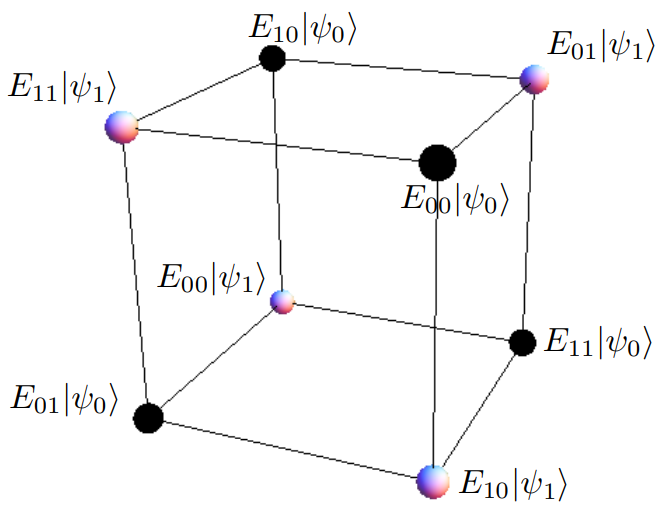
\includegraphics[width=0.5\linewidth]{Eightstatecube.png}
	\caption{A cube representing the eight cipherstates $E_{uw}\ket{\psi_{g}}$ as its corner points $(\pm1,\pm1,\pm1)^T/\sqrt{3}$ \cite{DeVries2016}.}
	\label{fig:eightstatecube}
	\end{center}
\end{figure}
\end{center}

\subsubsection{Diagrammatic Representation of Quantum Key Recycling}
We need to introduce some new diagrammatic notation for eight state encoding. After all, we need to move from a system of two bases to one of four. With that being said, a large part of it should be rather intuitive since we have essentially seen most of it already. The quantum one time pad is actually an eight state encryption protocol. The main difference is that in the protocol introduced for QKR, the eight states are distributed differently over the Bloch sphere. Diagrammatically, we can exploit the similarities by borrowing the notation that was previously introduced for the Bell maps in the QOTP. According to equation (\ref{equation:EightStatePaulis}), we only need to define the properties of one of the bases of eight state encoding and get the others for free by applying Bell maps to the states of this original basis. We choose the color red for this new basis. The red basis has the following two basis states: $E_{00}\ket{\psi_{0}} = \mathbb{I}\ket{\psi_{0}} = \ket{\psi_{000}}$ and $E_{00}\ket{\psi_{1}} = \mathbb{I}\ket{\psi_{1}} = \ket{\psi_{001}}$. We should first define triangles that represent classical information on these states, similarly to how we have classical triangles for the gray and white bases. We use the color red for this as well. This gives us the following diagrammatic components for the preparation of a state and the effect in this basis.

\begin{equation}
	\label{equation:newbases}
	\ket{\psi_{00g}} \equiv \tikzfig{RedStatePrep} ~~~~~~ \bra{\psi_{00g}} \equiv \tikzfig{RedEffect}
\end{equation}

Note that we have as well that.

\begin{equation}
\label{equation:RedMeasureAndEffect}
\tikzfig{PrepAndMeasureRed} \equiv \delta_{ij}
\end{equation}

Finally, we need to define a spider that encodes these $\ket{\psi_{000}}$ and $\ket{\psi_{001}}$ to the respective quantum states. In fact, since equation (\ref{equation:spidermultilegdecomposed}) is independent for the choice of basis, we can just copy it and exchange the white triangles for red ones.

\begin{equation}
	\label{equation:RedSpiderPrepareAndMeasure}
\tikzfig{spidermultilegred} \equiv \tikzfig{spidermultilegdecomposedred}
\end{equation}

By a combination of equations (\ref{equation:RedMeasureAndEffect}) and (\ref{equation:RedSpiderPrepareAndMeasure}) it is trivial to check that the red spider follows the spider rules as they are given in section \ref{spiders}. On the other hand, we have to tread carefully regarding its interaction with differently colored spiders, since we cannot exploit mutual unbiasedness.

We are now in principle ready to employ eight state encoding as it was proposed in \cite{DeVries2016} diagrammatically. Equation (\ref{equation:BellMap}) tells us how we can make Bell maps diagrammatically, and equation (\ref{equation:EightStatePaulis}) tells us that we can create all of our cipherstates by applying these Bell maps to the new basis states $\ket{\psi_{00g}}$ from equation (\ref{equation:newbases}). Defining a new color for each of the bases, we could thus encode all of our eight different cipherstates as follows.

\begin{equation}
	\label{equation:EightStateEncodingInFull}
	E_{uw}\ket{\psi_{00g}} = \tikzfig{EightStateEncodingInFullX} \equiv 
	\begin{cases}
	\tikzfig{STATEMIDRED} & \text{if} ~\{u,w\} = \{0,0\} \\
	\tikzfig{STATEMIDPINK} & \text{if} ~\{u,w\} = \{0,1\} \\
	\tikzfig{STATEMIDGREEN} & \text{if} ~\{u,w\} = \{1,0\} \\
	\tikzfig{STATEMIDBLUE} & \text{if} ~\{u,w\} = \{1,1\} \\
	\end{cases}
\end{equation}

Since the different bases will reappear quite often, we can save ourselves from unnecessarily complex diagrams by redefining each combination of $u$ and $w$ into a new spider, each with a different color, corresponding to the colors chosen for the different bases in equation (\ref{equation:EightStateEncodingInFull}). These eight state encoding spiders represent the four bases of eight state encoding in much the same way the gray and white spider represent the two bases of four state encoding.

%\footnote{Note that all four of these spiders accept red colored triangles because we defined all of them as Pauli's with respect to states in the red basis. The red basis has thus been given a privileged position among the four colors. This is in line with \cite{DeVries2016}, where the authors suggest to encode a classical '0' as $\ket{\psi_{000}}$ and a '1' as $\ket{\psi_{001}}$, and define the other states as Pauli's with respect to these.} 

\begin{equation}
	\label{equation:EncryptionOperators}
	\{u,w\} = \{0, 0\} \Leftrightarrow \tikzfig{RedEncoding} ~~~~~~ \{u,w\} = \{0, 1\} \Leftrightarrow \tikzfig{YellowEncoding}~~~~~~ \{u,w\} = \{1, 0\} \Leftrightarrow \tikzfig{GreenEncoding}~~~~~~ \{u,w\} = \{1, 1\} \Leftrightarrow \tikzfig{BlueEncoding}
\end{equation}

To make our lives easier, we introduce one more spider. This spider is actually nothing new, it is the set of the four spiders introduced in \ref{equation:EncryptionOperators}. Having this spider may come in handy whenever we want to make a statement that counts for all four of the colored spiders. Instead of making the same statement for each of the different spiders, we can then make it once for this new spider. We choose the color brown for this.

\begin{equation}
\label{equation:brownspiderset}
\tikzfig{BrownSpider} \equiv \{~\tikzfig{RedSpider},~ \tikzfig{GreenSpider},~ \tikzfig{OrangeSpider},~ \tikzfig{BlueSpider}\}
\end{equation}

Finally, we can do the same for triangles of all colors. A brown triangle thus represents the set of all colors of triangles. Using these new tools we can reduce equation (\ref{equation:EightStateEncodingInFull}) to:

\begin{equation}
\label{equation:EightStateEncodingInFullBrown}
(\ref{equation:EightStateEncodingInFull}) = \tikzfig{STATEMIDBROWN}
\end{equation}

Let's first see what our QKR protocol looks like in this new notation.

\begin{equation}
	\label{equation:QKRGeneralFirstIntroduced}
	\tikzfig{QKRGeneralX}
\end{equation}
\textit{Note that whenever there are multiple brown components in a diagram, this means that those components can be any color as long as they are the same.}

Alice and Bob respectively encode and measure in the same basis. Eve controls some map $\Phi$ and receives one of its outputs. We do not include the one-time pad $j$ or any of the other classical pre- and postprocessing here since we do not need it for this security proof. With this all set up we are in principle ready to develop a security proof for noiseless QKR, purely diagrammatically. Our security proof is very similar to the one proposed by Kissinger and Westerbaan in literature \cite{Kissinger2017}, where they prove security of four state QKD relying largely on the mutual unbiasedness of the gray and white bases. Although we do bring this mutual unbiasedness indirectly into our security proof as well by incorporating the Bell maps which consist of the gray and white spiders that we have seen before, we will extend this proof to also incorporate our four new non-mutually unbiased bases. As we will see, we will rely on gray and white spiders only through the use of these Bell maps..

Putting in the property that the quantum channels and maps exhibit no noise according to Alice and Bob is equivalent to saying that Eve goes undetected whenever Alice and Bob measure in the same basis. Since Eve represents the environment this can also be interpreted as the quantum channels being noiseless. We have already briefly discussed the security proof of Kissinger and Westerbaan in section \ref{QuantumKeyDistribution}, where we made the same statement for Alice and Bob using the gray and white bases in equation (\ref{QKDProofSetup}). In this section, we called this 'the noiseless case'. Noting that brown represents the set of four colors introduced in equation (\ref{equation:brownspiderset}), we can implement this statement for our four new bases as follows.

\begin{equation}
	\label{equation:coloredspiders}
	\tikzfig{QKRProofSetupX} = \tikzfig{wire} ~~~~ \land ~~~~ \tikzfig{QKRProofSetupGreenX} = \tikzfig{wire} ~~~~ \land ~~~~ \tikzfig{QKRProofSetupYellowX} = \tikzfig{wire} ~~~~ \land ~~~~ \tikzfig{QKRProofSetupBlueX} = \tikzfig{wire} ~~~~ \Leftrightarrow ~~~~ \tikzfig{QAaSBProofSetupReal1X} = 
\tikzfig{wire}
\end{equation}

With this as a starting point we can pre- and postcompose decoding and encoding maps respectively as follows.

\begin{equation}
	\label{equation:QKDSetupRed}
	\tikzfig{QKDProof1X} = \tikzfig{QKDProof2}
\end{equation}

Now we can purify the brown spiders in equation (\ref{equation:QKDSetupRed}) by doubling and discarding an extra output according to equation (\ref{equation:Purification}). Note that we can also, without loss of generality, state that $\Phi = \hat{V}$ since $\Phi$ already fits the definition of a purified state given in equation (\ref{equation:Purification}). This gives rise to the following diagrams.

\begin{equation}
	\label{equation:QKRProof4}
	\tikzfig{QKRProof4X} = \tikzfig{QKRProof4AX} \equaltext{(\ref{equation:discarding})} \tikzfig{QKRProof5X}
\end{equation}
\textit{Where $\hat{\psi}$ can be any normalized pure state.}

By applying the essential uniqueness of purification (the theorem introduced in section \ref{section:essentialuniqueness}) to equation \ref{equation:QKRProof4} we receive equation (\ref{equation:PurifiedQKR}). Note that since we discarded multiple outputs in equation (\ref{equation:QKRProof4}) we also have to apply the unitary U over multiple outputs.

\begin{equation}
	\label{equation:PurifiedQKR}
	\tikzfig{QKRProof6X} = \tikzfig{QKRProof7X}
\end{equation}

Deleting the first and third outputs of the LHS of equation (\ref{equation:PurifiedQKR}) gives the following.

\begin{equation}
	\tikzfig{QKRProof6AX} \equaltext{\ref{equation:spiderfusion}} \tikzfig{QKRProof6BX} \equaltext{(\ref{equation:boringspider})} \tikzfig{QKRProof6BXA}
\end{equation}

Doing the same to the RHS of equation (\ref{equation:PurifiedQKR}):

\begin{equation}
	\label{equation:passingvonthrough}
	 \tikzfig{QKRProof6BXA} = \tikzfig{QKRProof9X}
\end{equation}

Note that this holds for spiders of all colors of equation (\ref{equation:coloredspiders}). The following is thus also true for spiders of all these colors.

\begin{equation}
\label{equation:vrules}
	\tikzfig{QKRProof10X} \equaltext{(\ref{equation:passingvonthrough}), \ref{equation:spiderfusion}} \tikzfig{QKRProof11X} ~~~~~~~~~~~~~~~~~~ \tikzfig{QKRProof12X} \equaltext{(\ref{equation:passingvonthrough}), \ref{equation:spiderfusion}} \tikzfig{QKRProof13X}
\end{equation}

We can use this equation (\ref{equation:vrules}) to show that V separates. That is, the map itself splits up and leaves no connection between Eve's output and Alice and Bob's in- and outputs. Since V is just the undoubled version of $\Phi$ this then also implies that $\Phi$ separates in a similar fashion, which is what we wanted to achieve. Starting with V itself:

\begin{equation}
	\label{equation:v}
	\tikzfig{QKRSeperationProof1X}
\end{equation}

The strategy is to add something separated from the diagram in equation (\ref{equation:v}) and put V in there. We can just compose the creation and deletion of a random variable. Adding it to the diagram and writing one output of V a bit more suggestively:

\begin{equation}
	\label{equation:vwithpauli}
	(\ref{equation:v}) = \frac{1}{D}~
	\tikzfig{QKRSeperationProof2X}
\end{equation}

Now, we need some method to attach the separated part to the diagram temporarily such that we can move V through. It turns out that eight state encoding gives us a map that can do exactly this: the random Bell maps. Equation (\ref{equation:AliceWithBell}) already showed how a random Bell map can separate two parts of a diagram. We place it between the two diagrams in equation (\ref{equation:vwithpauli}).

\begin{equation}
\label{equation:movevthrough}
(\ref{equation:vwithpauli}) \equaltext{(\ref{equation:AliceWithBell})} \tikzfig{QKRSeperationProof3X} \equaltext{(\ref{equation:vrules})} \tikzfig{QKRSeperationProof4X}
\end{equation}

What we need now is some way to pass V through these Bell maps and the surrounding encoding and decoding maps. Let's have a closer look at just the encoding map and the subsequent random Bell map by applying some test state $g$ to it.

\begin{equation}
	\label{equation:RedSpiderRandomPauli}
	\tikzfig{QKRSeperationProof5X}
\end{equation}

So what we have here is a random Bell map, precomposed by any of the four encoding maps and a test state of the same basis. Since each of the four bases are just Bell maps with respect to one another, combining the encoding and random Bell maps actually selects one of the four bases to encode in at random. More explicitly, remember by equation (\ref{equation:EightStatePaulis}) that each of the cipherstates can be created by two Bell maps and the $\ket{\psi_g}$ basis states ($\ket{\psi_{uwg}} = B_1^w B_2^u\ket{\psi_{g}}$). Then applying a random Bell map ($B_1^n B_2^m~where~n~and~m~are~random$) to any of the cipherstates gives the following.

\begin{equation}
\label{equation:EncodingInRandomCipherstate}
B_1^nB_2^mB_1^uB_2^w\ket{\psi_{g}} = B_1^lB_2^p\ket{\psi_{g}} \equaltext{\ref{equation:EightStatePaulis}} \ket{\psi_{lpg}} ~(\text{where}~ l \equiv n \oplus u ~\text{and}~ p \equiv m \oplus w)
\end{equation}

Which, by randomness of $l$ and $p$, is a cipherstate encoded into a random one of the bases. Encoding a state into a cipherstate with a certain basis and then applying a random Bell map is thus equivalent to encoding this cipherstate into a random basis. We can find this diagrammatically too. Remember that equation (\ref{equation:EightStateEncodingInFull}) tells us how we can encode in any basis by applying two Bell maps with respect to a state in the red basis diagrammatically. The brown spider and state from equation (\ref{equation:RedSpiderRandomPauli}) can thus be replaced by a red spider and state, followed by two Bell maps. Looking just at this encoding part and the random maps that follow immediately after we thus get:

\begin{equation}
	\label{equation:composingtwopaulis} (\ref{equation:RedSpiderRandomPauli}) \equaltext{(\ref{equation:EightStateEncodingInFull}),(\ref{equation:EightStateEncodingInFullBrown})}
 \tikzfig{ComposingTwoPauli's}
\end{equation}
\textit{Note that the letters next to the spiders have no physical significance, and are only there to help visualize which spider refers to which random variable.}

The only ingredient that we are missing is some way to move Bell maps past one another. Mathematically, the fact that we can do this is evident from the anticommutative property of Pauli's. Anticommutativity implies that any two Pauli's $\sigma_i$ and $\sigma_j$ satisfy $\sigma_i\sigma_j = - \sigma_j\sigma_i$. Of course, this rule then also holds for the Bell maps. Diagrammatically we can commute Bell maps using the $k-k'$ commute rule from section \ref{section:kkcommute} as follows.

\begin{equation}
\label{equation:commutingpaulis}
\tikzfig{CommutingPauli's} \equaltext{\ref{equation:RandomXBitFlipProof}} \tikzfig{CommutingPauli's1} \equaltext{\ref{equation:kkcommuterule}} \tikzfig{commutingPauli's3} \equaltext{\ref{equation:RandomXBitFlipProof}} \tikzfig{CommutingPauli's4}
\end{equation}

Putting this back into equation \ref{equation:composingtwopaulis} and moving around some spiders gives:

\begin{equation}
	(\ref{equation:composingtwopaulis}) \equaltext{\ref{equation:spidermultilegdecomposed}} \sum\limits_{nm}\tikzfig{ComposingTwoPauli's2} \equaltext{\ref{equation:commutingpaulis}}
	\sum\limits_{nm}\tikzfig{ComposingTwoPauli's3} \equaltext{\ref{equation:spiderfusion}}
	\sum\limits_{nm}\tikzfig{ComposingTwoPauli's4}
	\equaltext{\ref{equation:spiderfusion}}
	\sum\limits_{nm}\tikzfig{ComposingTwoPauli's5}
\end{equation}

By equation (\ref{equation:xormap}) we know that the m and w here are xor'd by the gray spider and the n and u are xor'd by the white spider. We define $m \oplus w \equiv p$ and $n \oplus u \equiv l$, where randomness of m and n implies randomness of p and l. This gives:

\begin{equation}
	\label{equation:commutingpaulisresult}
	(\ref{equation:commutingpaulis}) = \sum\limits_{lp} \tikzfig{ComposingTwoPauli's6}
\end{equation}

Which is a cipherstate $g$ encoded into a random basis by equation (\ref{equation:EightStateEncodingInFull}).
%Incorporating (\ref{equation:EncodingInRandomCipherstate}) into equation (\ref{equation:RedSpiderRandomPauli}) we get the following:

\begin{equation}
	\label{equation:fourcolourspiders}
	(\ref{equation:commutingpaulisresult}) \equaltext{(\ref{equation:EightStateEncodingInFull})}
	 \frac{1}{4}\tikzfig{STATEMIDRED} +
	 \frac{1}{4}\tikzfig{STATEMIDGREEN} +
	 \frac{1}{4}\tikzfig{STATEMIDPINK}+
	 \frac{1}{4}\tikzfig{STATEMIDBLUE}	
\end{equation}

And thus we see that the encoding and subsequent Bell maps in equation (\ref{equation:RedSpiderRandomPauli}) actually encode some input state $g$ into a random one of the four bases. Also note that since $g$ was a brown triangle, this result is independent of the basis of the input state. Encoding into a certain basis and then applying a random Bell map thus has the same effect as applying a random one of the basis spiders. We can put this result into the relevant parts of equation (\ref{equation:movevthrough}) as follows.

\begin{equation}
	\label{equation:QKRSeperationProof}
	\tikzfig{QKRSeperationProof8X} \equaltext{(\ref{equation:fourcolourspiders})} \frac{1}{4}\tikzfig{QKRSeperationProof9AXA} + \frac{1}{4} \tikzfig{QKRSeperationProof9BXA} + \frac{1}{4} \tikzfig{QKRSeperationProof9CXA} + \frac{1}{4} \tikzfig{QKRSeperationProof9DXA}
\end{equation}

By undoubling the wire and using equation (\ref{equation:vrules}) we can then move V through all of these.

\begin{equation}
\label{equation:passingvthroughpauli}
\begin{aligned}
	 (\ref{equation:QKRSeperationProof}) \equaltext{(\ref{equation:doubledstate})} \frac{1}{4}\tikzfig{QKRSeperationProof9AX} + \frac{1}{4} \tikzfig{QKRSeperationProof9BX} + \frac{1}{4} \tikzfig{QKRSeperationProof9CX} + \frac{1}{4} \tikzfig{QKRSeperationProof9DX} \\ \equaltext{(\ref{equation:vrules})}
	 \frac{1}{4}\tikzfig{QKRSeperationProof9BAX} + \frac{1}{4} \tikzfig{QKRSeperationProof9BBX} + \frac{1}{4} \tikzfig{QKRSeperationProof9BCX} + \frac{1}{4} \tikzfig{QKRSeperationProof9BDX} \\
	 \equaltext{(\ref{equation:vrules})}
	  \frac{1}{4}\tikzfig{QKRSeperationProof10AX} + \frac{1}{4} \tikzfig{QKRSeperationProof10BX} + \frac{1}{4} \tikzfig{QKRSeperationProof10CX} + \frac{1}{4} \tikzfig{QKRSeperationProof10DX} \equaltext{(\ref{equation:fourcolourspiders})} \tikzfig{QKRSeperationProof11X}
\end{aligned}
\end{equation}

Finally, applying this to the larger picture.

\begin{equation}
	\label{equation:vpassingthrough}
	(\ref{equation:movevthrough}) = 
	\tikzfig{QKRSeperationProof4X} \equaltext{(\ref{equation:passingvthroughpauli})} \frac{1}{D}~ \tikzfig{QKRSeperationProof12X} \equaltext{(\ref{equation:AliceWithBell})}	\frac{1}{D}~ \tikzfig{QKRSeperationProof13X} \equaltext{\ref{equation:spiderfusion}} \frac{1}{D}~ \tikzfig{QKRSeperationProof14X}
\end{equation}

And thus we see that V splits up such that Alice's input is connected to Bob's output directly, and that Eve's output is completely separated from this. Hence, under the condition that Alice and Bob measure and encode in the same four bases from equation (\ref{equation:brownspiderset}) and see no disturbance or noise, $\Phi$ separates. In diagrams this as written as there existing some $\rho$ such that $\Phi$ separates as follows.

\begin{equation}
\label{equation:QKRSeparates}
\tikzfig{QKRSeperationProof15X} = \tikzfig{QKRSeperationProof16X}
\end{equation}

\section{Equivalences}
\label{Equivalences}

\subsection{QOTP and Quantum Teleportation}

The equivalence between QOTP and quantum teleportation is rather trivial. In fact, we already saw this equivalence back in equation (\ref{equation:QOTPQuantumTeleportationEquivalence}).

\begin{equation}
(\ref{equation:QOTPNoEve}) =
\tikzfig{QOTPNoEveNoLineXWithText} \equaltext{\ref{equation:spiderfusion}} \tikzfig{QOTPNoEveNoLine(1)}~~~~~ = \tikzfig{QuantumTeleportationNoLineWithText} =
(\ref{equation:quantumteleportation}) 
\end{equation}

This is a strikingly simple equivalence. Bending the U-shaped curve in the quantum teleportation protocol such that it becomes a straight line already does the trick. In a sense, quantum teleportation could thus be seen as the EPR variant of the QOTP. 

Due to their equivalence, whatever we can prove with the one diagram we can state as fact for the other without needing to prove it. This can be very convenient in security proofs.

\subsection{Protocol equivalences from the paper "Quantum Alice and Silent Bob" \cite{cryptoeprint:2019:875}}

\label{section:QAaSBEequivalences}
In a recent article \cite{cryptoeprint:2019:875}, $\check{\textrm{S}}$korić and Leermakers propose a scheme for QKR that includes no classical communication from Alice to Bob and only one bit from Bob to Alice. To prove its security, the authors modify the proposed protocol to one that is better suited for this in a series of steps that preserve security-wise equivalence to the original. In this section, we will have a look at these equivalences diagrammatically using the eight state encoding QKR protocol from equation (\ref{equation:QKRGeneral}) as starting point which we have proven secure in the noiseless case in section \ref{section:qkr}.

\begin{equation}
\label{equation:QKRGeneral}
	\tikzfig{QKRGeneralX}
\end{equation}


\subsubsection{Masking the qubit payload with public randomness}
\label{section:maskingqubitpubrand}
In the first equivalent protocol Alice and Bob both xor the same bitstring $a \in \{0,1\}^n$ in the classical domain with their payload and measurement result respectively. $a$ is public, implying that Eve also learns it. The rest of the protocol remains the same. To implement this diagrammatically, we give Eve another map with respect to (\ref{equation:EveNewMap}) to represent her doing classical post processing. In this map, she uses her knowledge on $a$ and what she learned from intercepting the quantum state from Alice to Bob. We could also include this map later on. However, since we have to include it anyway we may as well do it here already, such that we can avoid to introduce it along with the more complicated equivalences that are to follow.

We need to create one more set of maps before we can implement this diagrammatically. Since we haven't fully worked out all of the properties of the colored spiders yet, it is more convenient to not use them whenever the protocol doesn't tell us to. Therefore, we propose a map that translates between the white and colored bases. This allows us to do all of the classical processing in terms of white and gray spiders which is necessary if we want to use, for example, mutual unbiasedness (\ref{complementarity}) or the xor map (\ref{xorgate}). The map that translates between the white and red bases is the following.

\begin{equation}
\label{equation:EightStateSpider}
\tikzfig{EightStateSpider} :
\ket{g}_z \mapsto \ket{\psi_{00g}} ~~~~ \tikzfig{REightStateSpider} :
\ket{\psi_{00g}} \mapsto \ket{g}_z
\end{equation}

The other three colors then also have the respective boxes.

\begin{equation}
\label{equation:EightStateSpiderGreen}
\tikzfig{EightStateSpiderGreen} :
\ket{g}_z \mapsto \ket{\psi_{10g}} ~~~~ \tikzfig{REightStateSpiderGreen} :
\ket{\psi_{10g}} \mapsto \ket{g}_z
\end{equation}

\begin{equation}
\label{equation:EightStateSpiderOrange}
\tikzfig{EightStateSpiderOrange} :
\ket{g}_z \mapsto \ket{\psi_{01g}} ~~~~ \tikzfig{REightStateSpiderOrange} :
\ket{\psi_{01g}} \mapsto \ket{g}_z
\end{equation}

\begin{equation}
\label{equation:EightStateSpiderBlue}
\tikzfig{EightStateSpiderBlue} :
\ket{g}_z \mapsto \ket{\psi_{11g}} ~~~~ \tikzfig{REightStateSpiderBlue} :
\ket{\psi_{11g}} \mapsto \ket{g}_z
\end{equation}

We call these maps the eight state encryption maps. Again, the brown box is the set of the four individual maps.

\begin{equation}
	\label{brownbox}
	\tikzfig{EightStateSpiderBrown} \equiv \{ ~\tikzfig{EightStateSpider}, ~\tikzfig{EightStateSpiderGreen}, ~\tikzfig{EightStateSpiderOrange}, ~\tikzfig{EightStateSpiderBlue}\}
	~~~~~~~~~
	\tikzfig{REightStateSpiderBrown} \equiv \{ ~\tikzfig{REightStateSpider}, ~\tikzfig{REightStateSpiderGreen}, ~\tikzfig{REightStateSpiderOrange}, ~\tikzfig{REightStateSpiderBlue}\}
\end{equation}

The maps on the right side of equation (\ref{brownbox}) can be summarized in Dirac notation as $G_{uw}$. 

\begin{equation}
G_{uw} \equiv \ket{0}_z\bra{\psi_{uw0}} + \ket{1}_z\bra{\psi_{uw1}}
\end{equation}

And the maps on the left side are then of course summarized as the Hermitian adjoint of $G_{uw}$, $G_{uw}^\dagger$.

\begin{equation}
G_{uw}^\dagger \equiv \ket{\psi_{uw0}}\bra{0}_z + \ket{\psi_{uw1}}\bra{1}_z
\end{equation}

Since $G_{uw} \neq G_{uw}^\dagger$ the brown box is not self-adjoint and due to the complex elements in $\ket{\psi_{uwg}}$ it is not self-conjugate either. This is why we chose to give the eight state encryption maps a shape in which their orientations can easily be determined. We also know that they are unitary:

\begin{equation}
G_{uw}G_{uw}^\dagger = \ket{0}_z\bra{0}_z + \ket{1}_z\bra{1}_z = \mathbb{I} \Leftrightarrow \tikzfig{UnitarySmllBrownBox} = \tikzfig{wire}
\end{equation}

Including these maps, and the fact that Alice and Bob both xor with a public variable $a$ in their classical domain, we have the following diagram.

\begin{equation}
	\label{equation:QKRQAaSBA1}
	\tikzfig{QKRQAaSBA1X}
\end{equation}
\textit{With $\Phi_1$ the map that Eve uses to intercept the communication and $\Phi_2$ the map that Eve uses to do classical processing on both this intercepted data and $a$.}

%The central part of this diagram - Eve's map $\Phi_1$ and the %encoding and measuring operations by Alice and Bob - we have already %seen (\ref{equation:coloredspiders}). This is the QKR protocol which %we have proven secure in section \ref{section:qkr}.
For a security proof of this protocol, we can state that Eve's operations introduce no noise from Alice and Bob's perspective whenever they measure in the same basis. This is the same statement that we made in section \ref{section:qkr} to prove the security of QKR, and in section \ref{QuantumKeyDistribution} to prove the security of QKD, where we referred to this as the 'noiseless case'. For the diagram in equation (\ref{equation:QKRQAaSBA1}), this looks as follows.

\begin{equation}
\label{equation:QAaSBProofSetupReal}
\tikzfig{QKRQAaSBA1DiscardingEveX} = ~~ \tikzfig{longwire}
\end{equation}

By causality we then know that applying Eve's map $\Phi_2$ and then deleting its output is essentially the same as not having applied Eve's map altogether. In other words, from Alice and Bob's perspective, there is no difference between deleting the output of Eve's map $\Phi_2$ or deleting its inputs even before she applies it. Therefore equation (\ref{equation:QAaSBProofSetupReal}) reduces to:

\begin{equation}
\label{equation:QKRQAaSBA1DiscardingEve1}
\tikzfig{QKRQAaSBA1DiscardingEve2X} 
=\tikzfig{longwire}
\end{equation}

Then we can pre and postcompose another xor with $a$ on both sides of equation (\ref{equation:QKRQAaSBA1DiscardingEve1}).

\begin{equation}\\
\label{equation:QKRQAaSBA1DiscardingEve3}
\tikzfig{QKRQAaSBA1DiscardingEve3X} = ~~ \tikzfig{longwire1X} ~
\Leftrightarrow
\tikzfig{QKRQAaSBA1DiscardingEve4X} = ~~ \tikzfig{longwire2X}
\end{equation}

According to the diagrammatic rules for mutual unbiasedness given in equation (\ref{equation:Complementarity}) this separates $a$ on both sides of equation (\ref{equation:QKRQAaSBA1DiscardingEve1}).

\begin{equation}
\label{QKRQAaSBA1DiscardingEve5}
\tikzfig{QKRQAaSBA1DiscardingEve5X} = ~~ \tikzfig{longwire3X}
\end{equation}

Which is equivalent to the same diagrams without a random $a$.

\begin{equation}
\tikzfig{QKRQAaSBA1DiscardingEve6X} = ~~ \tikzfig{longwire4} ~~ \equaltext{\ref{equation:boringspider}} ~~ \tikzfig{longwire}
\end{equation}

Finally, postcomposing a brown eight state encryption map, precomposing its adjoint and exploiting the fact that it is unitary:

\begin{equation}
\tikzfig{QKRQAaSBA1DiscardingEve8X} = ~~ \tikzfig{longwire5} ~ \Leftrightarrow ~~ \tikzfig{QKRQAaSBA1DiscardingEve9X} = ~~ \tikzfig{wire}
\end{equation}


This equation we have already seen, it is the starting point for the security proof of eight state encoding QKR, equation (\ref{equation:QKDSetupRed}).\footnote{There is of course a minor difference: In (\ref{equation:QKDSetupRed}) Eve has the map $\Phi$ and here Eve has the map $\Phi_1$. This is insignificant however. $\Phi_1$ was only introduced to distinguish between Eve's quantum map and Eve's classical map. We can just say that $\Phi$ = $\Phi_1$ without loss of generality since Eve's quantum map can be any (multitude of) unspecified operation(s) in both cases.} Therefore, we could just follow all the steps which we followed in section \ref{section:qkr} and get as a result that $\Phi_1$ separates as follows.

\begin{equation}
	\label{equation:QKRGeneralSeparation}
	\tikzfig{QKRGeneralQAaSBNoMeasuringX} = \tikzfig{QKRGeneralQAaSBSeparatedX}
\end{equation}

This is why this protocol is security-wise equivalent to the starting point of the equivalences, equation (\ref{equation:QKRGeneral}), it relies on the same security proof. If it turns out that the security proof in section \ref{section:qkr} for the original QKR protocol only allows for security up to some factor, the protocol with public randomness from this section is also only secure up to that same factor. Putting this back into equation (\ref{equation:QKRQAaSBA1}) we get the following:

\begin{equation}
	\tikzfig{QKRQAaSBA1NoDottedLineX} \equaltext{\ref{equation:QKRGeneralSeparation}} \tikzfig{QKRQAaSBA2X}
\end{equation}

In a series of steps following rules which we have seen before we can show that Eve's map again separates entirely from Alice and Bob's part of the diagram.

\begin{equation}
	\begin{aligned}
	\tikzfig{QKRQAaSBA3X} \equaltext{\ref{equation:EightStateSpider}} \tikzfig{QKRQAaSBA4X} \equaltext{\ref{equation:spiderfusion}} \tikzfig{QKRQAaSBA5X} \\ \equaltext{\ref{doubling}} \tikzfig{QKRQAaSBA6X} \equaltext{\ref{equation:Complementarity}} \tikzfig{QKRQaASBA7X} = \tikzfig{QKRQAaSBA8X}
	\end{aligned}
\end{equation}

So we see that even though Eve gets $a$ and some quantum state, she is not attached to Alice and Bob's communication channel. Alice and Bob on the other hand achieve uninterrupted communication. This is what we would intuitively expect for the noiseless case. 

\subsubsection{EPR version of the protocol}

\label{section:eprqkr}
The second equivalent protocol is an EPR version of the original. We have already seen a diagrammatic implementation of an EPR protocol in section \ref{subsection:QuantumTeleportation}, the diagram for quantum teleportation. The characteristic difference between an EPR version of a protocol and a normal version is that in the former Alice and Bob share some entangled qubit. In quantum teleportation this is the Bell state $B_0$, given by the doubled wire shaped like a cup in equation (\ref{equation:quantumteleportation}).

Diagrammatically, it is rather trivial to go from the protocol introduced in the previous section (\ref{equation:QKRQAaSBA1}) to an EPR version. In fact, we only need to bend around some wires. We split this up in a few steps to show where all the parts go. First of all, bending around Alice's wire according to the yanking equation (\ref{equation:yankingequation}):

\begin{equation}
	\label{equation:QAaSBEPREquivalence}
	\begin{aligned}
	\tikzfig{QKRQAaSBA1NoDottedLineX} \equaltext{\ref{equation:yankingequation}} \tikzfig{QKRQAaSBB2X}
	\end{aligned}
\end{equation}

Subsequently pulling her encoding and encryption operations through:

\begin{equation}
\label{equation:EPRQKR}
	\begin{aligned}
 (\ref{equation:QAaSBEPREquivalence}) = \tikzfig{QKRQAaSBB3X} = \tikzfig{QKRQAaSBB4DottedLineX}
\end{aligned}
\end{equation}

Which is indeed the EPR version of the protocol in equation (\ref{equation:QKRQAaSBA1}).

\begin{equation}
\label{equation:QKRQAaSBB4DottedLine}
	(\ref{equation:EPRQKR}) = \tikzfig{QKRQAaSBB4DottedLineX} = \tikzfig{QKRQAaSBA1X} = (\ref{equation:QKRQAaSBA1})
\end{equation}

Of course, if these protocols are equivalent, then by security-wise equivalence of (\ref{equation:QKRQAaSBA1}) and (\ref{equation:QKRGeneral}) we also have security-wise equivalence of the EPR version introduced in this section, (\ref{equation:EPRQKR}), and (\ref{equation:QKRGeneral}), the protocol that was the starting point of all these equivalences. 

\subsubsection{Adding a random permutation}

In the next equivalent step, the authors propose that Alice and Bob both publicly decide on the same random permutation ($\pi$) to apply to their own set of qubit states before measuring, and forget it right after. Eve, however, can remember this permutation. Diagrammatically, this looks as follows.

\begin{equation}
	\label{equation:QKRQAaSBC1}
	\tikzfig{QKRQAaSBC1X}
\end{equation}

Intuitively, it is evident that this step preserves equivalence to the original from Alice and Bob's perspective due to the fact that this steps preserves entanglement of the EPR states. Whether this protocol works or not for Alice and Bob is independent on the choice of states that they receive, as long as they are entangled. The states that Eve sends to Alice and Bob are entangled up to a certain degree dependent on the amount of noise Eve introduces, and the $\pi$'s completely preserve entanglement since the same operation is applied on both qubits. To make a diagrammatic proof from this intuition we have to first exploit the fact that we can turn Eve's map into a state. We can do this as follows.

\begin{equation}
\label{equation:QKRQAaSBC6}
\tikzfig{QKRQAaSBC1XA} = \tikzfig{QKRQAaSBC6X}
\end{equation}
\textit{Note that the dotted map in this diagram has no diagrammatic significance and is only intended for didactic purposes.}

We can show that this is a valid operation diagrammatically. Isolating just the state of Eve in the RHS of equation (\ref{equation:QKRQAaSBC6}) and realizing that Eve has the freedom to do whatever she wants in her state $\Phi_1$.

\begin{equation}
\label{equation:QKRQAaSBC7}
\tikzfig{QKRQAaSBC7} = \tikzfig{QKRQAaSBC8}
\end{equation}

Then using the yanking equation (\ref{equation:yankingequation}):

\begin{equation}
\label{equation:QKRQAaSBC9}
(\ref{equation:QKRQAaSBC7}) = \tikzfig{QKRQAaSBC9} \equaltext{\ref{equation:yankingequation}} \tikzfig{QKRQAaSBC10}
\end{equation}

We see that we can transform Eve's map into a state and reversedly. The operation from equation (\ref{equation:QKRQAaSBC6}) is therefore valid.

Starting with the RHS of equation (\ref{equation:QKRQAaSBC6}) and using the yanking equation (\ref{equation:yankingequation}):

\begin{equation}
\begin{aligned}
\label{equation:QKRQAaSBC11}
 (\ref{equation:QKRQAaSBC6}) = \tikzfig{QKRQAaSBC11X} \equaltext{\ref{equation:yankingequation}} \tikzfig{QKRQAaSBC12X}
\end{aligned}
\end{equation}

Now we are ready to put in the intuition that we had in the beginning of this section. From Alice and Bob's perspective, everything they need is for Eve to prepare and send them an (imperfect) EPR state. If Eve does this in her map $\Phi_1$ the two subsequent random permutations will potentially change the particular choice of EPR states that Alice and Bob receive, but they will remain entangled since the same operation is applied on both sides. Furthermore, Alice and Bob forget $\pi$ right after they apply it. Therefore, after it is applied, they are indifferent for as to whether they did it or Eve did it. From Eve's perspective, it does not matter whether she applies these $\pi$'s or whether Alice and Bob apply them. She knows the $\pi$'s that are applied in both cases. Taking this into account, we realize that we can just 'shove' the $\pi$'s into Eve's state and assume that she applied them rather than Alice and Bob. From a security perspective, this is an operation that preserves equivalence. 

\begin{equation}
	\label{equation:QKRQAaSBC13}
	(\ref{equation:QKRQAaSBC11}) = \tikzfig{QKRQAaSBC12AX} = \tikzfig{QKRQAaSBC13X}
\end{equation}

To show that this protocol is equivalent to the protocols from the previous sections we can just turn Eve's state back into a map.

\begin{equation}
\label{equation:QKRQAaSBBFinalResult}
	\tikzfig{QKRQAaSBC13XA} \equaltext{(\ref{equation:QKRQAaSBC9})} \tikzfig{QKRQAaSBC14X} \equaltext{(\ref{equation:QKRQAaSBC9})} \tikzfig{QKRQAaSBB3X} = (\ref{equation:EPRQKR})
\end{equation}

And so we see that the protocol from this section is equivalent to the protocol of the previous section, equation (\ref{equation:EPRQKR}), and therefore indirectly also to (\ref{equation:QKRGeneral}), the starting point of this series of equivalences.

\subsubsection{Adding random Pauli transforms}

In the final equivalent step, the authors propose that Alice and Bob both publicly decide on the same random Pauli to apply to their own qubit states before measuring. Afterwards they again forget about their particular choice of Pauli. Remembering the equivalence between the Pauli's and the Bell maps from equation (\ref{equation:bellsigmas}) and how to construct Bell maps from equation (\ref{equation:BellMap}), this looks as follows.

\begin{equation}
\label{equation:QKRQAaSBD1}
\tikzfig{QKRQAaSBD1X}
\end{equation}

The difference between this protocol and the EPR protocol introduced in section \ref{section:eprqkr} are the two single spiders in the middle which represent the classical random variables that determine the Bell maps which are applied to both Alice and Bob's states. Information on the particular choice of Bell maps also goes to Eve by the thin lines originating from these two single spiders. Let's isolate the Bell map that Alice gets and her measurement and eight state encryption maps.

\begin{equation}
	\label{equation:QKRPauli's}
	\tikzfig{QKRPauli's1X} \Rightarrow \tikzfig{QKRPauli's2X} \equaltext{\ref{equation:spidermultilegdecomposed}} \sum\limits_{nm} \tikzfig{QKRPauli's3}  \equaltext{\ref{equation:spidermultilegdecomposed}} \sum\limits_{nm} \tikzfig{QKRPauli's4}
\end{equation}

We do not consider the two triangles that go to Bob for now. These simply determine the Bell maps that he applies to his qubit state. All we need to know is that they are the same as Alice's. Furthermore we can take the brown decoding spider of Alice further apart according to equation (\ref{equation:EightStateEncodingInFull}). This equation shows how all the cipherstates can be encoded by a red spider and two Bell maps. Since decoding is the adjoint of decoding, we can decode in any of the four bases by first applying two Bell maps followed by a red spider. To then return back to the classical z basis we need to also exchange the brown eight state encryption box for a red one.

\begin{equation}
	\label{equation:QKRQAaSBD3}
	(\ref{equation:QKRPauli's}) \equaltext{\ref{equation:EightStateEncodingInFull}} \sum\limits_{nm}\tikzfig{QKRQAaSBD3}
\end{equation}

This equation is very similar to equation (\ref{equation:composingtwopaulis}). In fact, for equation (\ref{equation:composingtwopaulis}) we showed that encoding in a certain basis and then applying a random Bell map results in encoding in a random basis. Here we will show that applying a random Bell map and then decoding in a certain basis results in decoding in a random basis.

\begin{equation}
\label{equation:QKRQAaSBD4}
(\ref{equation:QKRQAaSBD3}) \equaltext{\ref{equation:commutingpaulis}} \sum\limits_{nm}\tikzfig{QKRQAaSBD4} \equaltext{\ref{equation:spiderfusion}} \sum\limits_{nm}\tikzfig{QKRQAaSBD5} \equaltext{\ref{equation:spiderfusion}} \sum\limits_{nm}\tikzfig{QKRQAaSBD6} 
\end{equation}

By equation (\ref{equation:xormap}) we know that the gray n and u are xor'd by the white spider and that the white m and w are xor'd by the gray spider. Defining $m \oplus w \equiv p$ and $n \oplus u \equiv l$ and realizing that l and p are random then gives:

\begin{equation}
	\label{equation:randompaulidecoding}
	(\ref{equation:QKRQAaSBD4}) = 
	\sum\limits_{nmlp}\tikzfig{QKRQAaSBD7} \equaltext{\ref{equation:spideroneoutput}} \sum\limits_{lp}\tikzfig{QKRQAaSBD8}
\end{equation}

As expected, Eve receives the random variables n and m, but she does not learn l and p since these require knowledge of u and w. Alice and Bob thus measure in a random basis and Eve doesn't know this basis. More importantly for Alice and Bob, they measure in the same random basis since for Bob's side, the whole derivation follows the same series of steps. Putting this back into the larger picture, equation (\ref{equation:QKRQAaSBD1}):

\begin{equation}
	\label{equation:QKRQAaSBDResult}
	\begin{aligned}
	(\ref{equation:QKRQAaSBD1}) \equaltext{\ref{equation:randompaulidecoding}}
	\sum\limits_{lp}\tikzfig{QKRQAaSBD12X} 
	=
	 \frac{1}{4}\tikzfig{QKRQAaSBDResultRX} \\+
	\frac{1}{4}\tikzfig{QKRQAaSBDResultGX} +
	\frac{1}{4}\tikzfig{QKRQAaSBDResultOX} +
	\frac{1}{4}\tikzfig{QKRQAaSBDResultBX}
	\end{aligned}
\end{equation}

Each of these protocols occur with probability $\frac{1}{4}$. We also know that they are all security-wise equivalent to the protocol in equation (\ref{equation:EPRQKR}) since they form the members of the set of protocols in the RHS of equation \ref{equation:EPRQKR}. The protocol in equation (\ref{equation:QKRQAaSBD1}) thus preserves security-wise equivalence to the protocol that was the starting point of this series of equivalences, equation (\ref{equation:QKRGeneral}).

\section{Discussion}
\label{section:discussion}


% Talk about aims, were they achieved? Good conclusion paragraph. Combining summary with talk about aims, should I do this?


After reading up to this point, the novelty of this research may not be self-evident. After all, we did not develop any new protocols or give higher security bounds on existing protocols. Be that as it may, these are not the kind of things that should be expected of the diagrammatic method as of yet. The novelty of this work comes from the fact that it provides diagrammatic realizations of protocols and security proofs that have never been worked out in this fashion before. We took preexisting work and gave it a place in the context of the diagrammatic method for quantum cryptography. As of now it is not yet the task of the diagrammatic method to develop novel protocols or provide higher security bounds. Before we could do any of that, we should first see whether and how we can work up to the current state of the art diagrammatically. Only when and if we reach that point, we can attempt to use this method to actually bring the field of quantum cryptography further. This work provides a foundation to reach this point. Kissinger and Westerbaan built this foundation for quantum key distribution in \cite{Kissinger2017} and in this work we did the same for quantum key recycling with eight state encoding and the (quantum) one time pad.

With that being said, maybe it is not even the role of the diagrammatic method to eventually provide new protocols or bounds on security proofs. Coecke and Kissinger - in their first book on this method - propose it to be fully independent as an alternative to Dirac notation. Their book aims to give a first introduction into quantum mechanics, where new topics are introduced along with the notation and no knowledge of Dirac notation is assumed. Since this works well, the notation allows for a satisfactory representation of the introductory concepts of quantum mechanics. The question then arises of whether it also allows for the representation of more advanced quantum mechanical topics, in particular in the field of quantum cryptography. In this report, we take it a bit further than in the book of Coecke and Kissinger. We use the diagrammatic method to make security proofs and analyze some recent papers' equivalences. We do at no point, however, assume that Eve introduces noise since whenever we would do this, we would introduce more advanced equations for which we have not worked out the diagrammatic notation yet. Kissinger and Westerbaan in \cite{Kissinger2017} do not shy away from combining the notation with such equations in their security proof for QKD with noise. With that being said, their approach is a bit clumsy since they remove the need for diagrams by using these equations. Their security proof by itself is also not state of the art. It is mostly relevant since it is the first security proof for QKD that is conducted mostly with the diagrammatic notation. Therefore the question remains whether this notation should really be used for tasks such as making rigorous security proofs or the development of new and improved protocols. So far it does not seem very suitable for this task. With that being said, it is a relatively new method - Coecke and Kissinger released their book in 2017 \cite{Coecke2017} - so it may in the future take up more responsibility. What we can say about it as of now is that it is a good notation for intuitively displaying protocols and a very useful method for visualizing their equivalences. The equivalence between the QOTP and quantum teleportation, for example, is not that straightforward just from reading the text, but is strikingly simple diagrammatically. 

The critique that we can give to this method also depends on the role that it takes up. If we assume that the role of the diagrammatic method is to give in-depth security proofs for noisy protocols with advanced statistics, we could easily say that the notation is not rigorous enough. Under this assumption, it would have to be developed further to be relevant. If we assume, on the other hand, that the role of the diagrammatic method is to draft up and intuitively display proofs and equivalences, we would have to be much less critical. The latter is therefore also the role that we assume it will have in future work. A cause for confusion of this notation though, independent of its role, is the fact that single wires have a basis. Interpreting single wires as classical data is not very intuitive. Bits are not encoded into bases. A better way to interpret single wires is then as carriers of 'classical data on how to encode a qubit in a certain basis'. However, in this case every wire would carry around some information on what color it is in. This is not how wires are represented in this notation, they do not have a color. Coecke and Kissinger identify this problem as well in their book \cite{Coecke2017} on page 740, where they propose to place a small square next to each wire to show the basis of the information that it carries. 

\begin{equation}
	\tikzfig{explicitgraywire} ~~~~~~~~~~~~~~ \tikzfig{explicitwhitewire}
\end{equation}

On the one hand, including this in the notation would make it more rigorous. There would be no confusion anymore on the basis of the information carried by each wire. On the other hand, it would remove a lot of the elegance and simplicity of the notation. It would probably be good to use this notation whenever the basis of the information carried by a wire is not clear from context, and to omit it otherwise.

This work leaves open plenty of opportunities for future research. As a direct follow up to this report, a noisy version of the quantum key recycling security proof could be developed. It is probable that a security proof along the lines of the one for noisy quantum key distribution given in \cite{Kissinger2017} also applies to the QKR protocol from section \ref{section:qkr}. Furthermore, since the diagrammatic method is very young and literature on it is scarce, it would benefit from more protocols and their security proofs being written out in this fashion.

\section{Conclusion}
\label{section:conclusion}
% Summary
The aim of this research was largely divided up into two parts. The first was to introduce the reader to the diagrammatic method in a concise manner. Therefore, chapter \ref{section:preliminaries} functions as a sort of handbook to the diagrammatic notation for a reader familiar with undergraduate level quantum mechanics. Although all the necessary concepts were introduced and derived back to Dirac notation successfully, whether this fully satisfied this aim or not is up to the reader to decide. Secondly, this research aimed to place this notation into the relevant quantum cryptographic context. To this end, we worked out four protocols and their security diagrammatically, and also used the notation to represent a series of equivalences. In particular for quantum key recycling we developed new notation for eight state encoding, a concept that was recently introduced by $\check{\textrm{S}}$korić and De Vries \cite{DeVries2016}. Furthermore we gave a security proof for eight state QKR in a similar fashion to how it was done for QKD in \cite{Kissinger2017}. The equivalences that we worked out diagrammatically come from another publication \cite{cryptoeprint:2019:875}. In this research, the authors provide a series of security-wise equivalent steps, allowing them to prove security of one protocol indirectly by proving the security of another. We went through each of these steps diagrammatically, which allowed for both their formal proof and an intuitive understanding of these equivalences. With all of this taken into account, it can be said that this second aim - to build upon the novel notation and use it to add relevant research to the field of quantum cryptography - was successfully achieved. This work does leave open significant questions about the role of the diagrammatic method in the field of quantum cryptography though. We conclude that the diagrammatic notation should not be used for its rigorosity, but rather for its capability to intuitively describe protocols and their equivalences. In future work, a noisy version of QKR could be developed. In the larger context, the notation would benefit from being implemented in more protocols and their respective security proofs.

%In general, this self-contained work brings the reader in an intuitive manner from undergraduate level quantum mechanics to understanding some recent articles on quantum cryptography from a diagrammatic perspective. Therefore, it could form a compelling argument for researchers in the field of quantum cryptography to use this notation for their own research. 

\section{Critical reflection}
\label{section:criticalreflection}
In general, I would say that I am very satisfied with the project and its results. Of course, there are some points of critique and general thoughts to keep in mind for future projects that I can come up with.

\subsection{Organization of tasks}

At the start of the project I had many ideas about how to organize the project and optimize the time I had for communication with my supervisors. One of them, for example, was to use a Kanban board that my supervisors could access as well to organize tasks. This Kanban board was useful in the beginning of the project when I was defining the scope and assessing what needed to be done. However, after a couple of weeks I found myself looking at the board only rarely. Although I did not get any feedback on this, I do not think my supervisors measured my progress by the Kanban board either. I forced myself to keep using it for a while but decided to stop doing this completely after a couple of weeks. I noticed that after I stopped using it I naturally went into a cycle of making progress for a few weeks and writing for a week or two after I reached some milestone. At the end of each cycle, writing about it would finish that part of the work such that I could put it to the side and clear my mind to think about what task to take on next. This method of organizing tasks is mainly different from the use of a Kanban board in that there is no predefined set of tasks to follow; each task is made up only after the previous one is finished. I enjoyed working like this more and I think it also increased productivity. This is a pattern that I actually noticed more often. As I started to feel more comfortable in the project I started to organize tasks more naturally rather than by following some predefined framework. In general, this actually made the work more enjoyable and increased productivity. This is something that I will remember and try to take into account from the start in future projects.

%\subsection{Handling criticism}

%I don't think many people particularly enjoy receiving criticism on their work, myself included. With that being said, I try to be open to it so that I can learn how to deal with it and get used to it through exposure. In this project I asked for criticism on various occasions, for example when I asked my supervisors to read parts of my texts, or when I doubted if a certain approach to solving a problem was the correct one. Of course, on many occasions I did make mistakes, and received the appropriate critique. Almost all of the time the criticism was on things that were just plain wrong, or could clearly have been done better. These cases were easy to accept after the mistake was understood. In other cases, where there was no direct mistake or the mistake was not understood by me, it was a bit more difficult to just accept the criticism. In the cases where I didn't understand the mistake I tried to ask for further explanation. In the cases where there was no direct mistake, but rather a stylistic suggestion for example, I mostly relied on the expertise and experience of my supervisors, and just implemented the suggestion. I think this was the correct thing to do. Although I only remember it happening very few times, it mostly turned out later that the supervisor's suggestions were the better choice in the long run.

\subsection{Listening while taking up information}
\label{section:listeninginfo}
Listening while taking up information was probably the most difficult aspect of the practical work of the thesis. I had many interesting and educative conversations with my supervisors and others who were doing research in the same field - something I actually did not expect to happen due to the limited amount of available time that academics tend to have. In the beginning, I used to write down as much as I could during these conversations such that afterwards I would be able to recall the points and actually implement them in the thesis. However, I noticed that these conversations actually became more fruitful after I stopped writing down so much because that gave me more time to both listen and think about a response or follow-up question. The downside of this was that I would sometimes forget points that were made during the conversation. In the end, I chose to write down very little, but would try to write down a keyword for each main discussed point. Although this worked quite well, I would still sometimes forget some details and I think the conversations still suffered from it a little. There are of course other options, such as recording the conversation. However, I cannot expect everyone to be comfortable with this, and this would probably also not be completely appropriate in more informal settings such as during lunch. I still do not know the optimal way to tackle this problem but I think that writing down just the main points while listening very closely is a good compromise. In the future I may also try to take some time right after each conversation, when memory of it is still fresh, to write down a summary of what was discussed.

\subsection{Putting things in perspective}

Sometimes I have trouble putting things in perspective. This is something that I was actually not aware of before or during the project, but was told to me afterwards by my research supervisor. After receiving this feedback I reread some parts with this in mind and I think I understand were this comes from. Firstly, I could have explicitly taken some more time to develop an understanding of the context but I chose to focus more on my own research and the papers that were directly relevant to it. Secondly, I think that experience in the field helps to place a work like this in the larger context. This experience gives a better view of what has come before, what research is being done currently, and what the likely paths are for the future. I had people around me who were much more experienced in the field, and who did possess knowledge of the larger context. For example, my research supervisor and his PhD student have multiple articles on QKR, one of the main subjects of this thesis. With them, I often discussed how this work could be put in the relevant perspective. I think what went wrong here relates to the previous section, \ref{section:listeninginfo}. Although we did talk much about how specific parts of this work could be put in perspective, it is not what I thought I should take away from these conversations. What I did try to remember from these conversations were usually more technical and tangible points since these were the kinds of things that I could put directly into words and diagrams after such a conversation. In the future I would approach this differently. I think the solution that I proposed before in \ref{section:listeninginfo} - to write a small summary after each conversation - would work well, provided I write about what was discussed about the larger context as well.

\bibliographystyle{plain}
\bibliography{library}
\appendix

% Summary, "Philosophical implications", what to do in future

\section{Keywords}
\label{Keywords}


~~~~\hyperref[coloursandbases]{Base, page 7}

\hyperref[section:basisandphasetranslations]{Bloch sphere, page 10}

\hyperref[braandket]{Bra, page 2}

\hyperref[coloursandbases]{Color, page 7}

\hyperref[complementarity]{Complementarity, page 11}

\hyperref[encodingdecoding]{Decoding, page 11}

\hyperref[spiders]{Deleting, page 6}

\hyperref[doubling]{Density matrix, page 8}

\hyperref[discarding]{Discarding, page 9}

\hyperref[doubling]{Doubling, page 7}

\hyperref[braandket]{Effect, page 2}

\hyperref[encodingdecoding]{Encoding, page 11}

\hyperref[entanglement]{Entangled state, page 9}

\hyperref[section:essentialuniqueness]{Essential uniqueness of purification, page 12}

\hyperref[discarding]{Fully mixed state, page 9}

\hyperref[braandket]{Hermitian Adjoint, page 3}

\hyperref[braandket]{Hermitian Conjugate, page 3}

\hyperref[identity]{Identity, page 3}

\hyperref[section:kkcommute]{$k-k'$ commute rule, page 13}

\hyperref[braandket]{Ket, page 2}

\hyperref[spiders]{Kronecker delta, page 5}

\hyperref[maps]{Linear map, page 4}

\hyperref[maps]{Map, page 5}

\hyperref[doubling]{Mixed state, page 8}

\hyperref[phasespiders]{Phase, page 6}

\hyperref[phasespiders]{Phase spider, page 6}

\hyperref[discarding]{Purification, page 9}

\hyperref[doubling]{Purity, page 8}

\hyperref[spiders]{Random variable, page 6}

\hyperref[spiders]{Spider, page 5}

\hyperref[braandket]{State, page 2}

\hyperref[identity]{System type, page 4}

\hyperref[section:tensorproduct]{Tensor product, page 3}

\hyperref[discarding]{Trace, page 9}

\hyperref[braandket]{Transpose, page 3}

\hyperref[identity]{Wire, page 3}

\hyperref[xorgate]{Xor map, page 12}

\hyperref[section:yankingequations]{Yanking equations, page 10}

\section{Bell and Pauli matrices}
\label{appendix:BellMaps}


The Bell maps are represented by the following matrices:

\begin{equation}
\begin{aligned}
B_0 = \sigma_0 = 
\begin{pmatrix}
1 & 0 \\
0 & 1
\end{pmatrix}  % top-left
~~~~&~~~~ B_1 = \sigma_1 =
\begin{pmatrix}
0 & 1 \\
1 & 0
\end{pmatrix}% top-right
% Want to start a new line here...
\\\\
B_2 = \sigma_3 =
\begin{pmatrix}
1 & 0 \\
0 & -1
\end{pmatrix}  % bottom-left
~~~~&~~~~  B_3 = i\sigma_2 =
\begin{pmatrix}
0 & -1 \\
1 & 0
\end{pmatrix}
\end{aligned}
\end{equation}


\end{document}
